% Options for packages loaded elsewhere
\PassOptionsToPackage{unicode}{hyperref}
\PassOptionsToPackage{hyphens}{url}
%
\documentclass[
]{article}
\usepackage{amsmath,amssymb}
\usepackage{lmodern}
\usepackage{iftex}
\ifPDFTeX
  \usepackage[T1]{fontenc}
  \usepackage[utf8]{inputenc}
  \usepackage{textcomp} % provide euro and other symbols
\else % if luatex or xetex
  \usepackage{unicode-math} % this also loads fontspec
  \defaultfontfeatures{Scale=MatchLowercase}
  \defaultfontfeatures[\rmfamily]{Ligatures=TeX,Scale=1}
\fi
\usepackage{lmodern}
\ifPDFTeX\else
  % xetex/luatex font selection
\fi
% Use upquote if available, for straight quotes in verbatim environments
\IfFileExists{upquote.sty}{\usepackage{upquote}}{}
\IfFileExists{microtype.sty}{% use microtype if available
  \usepackage[]{microtype}
  \UseMicrotypeSet[protrusion]{basicmath} % disable protrusion for tt fonts
}{}
\makeatletter
\@ifundefined{KOMAClassName}{% if non-KOMA class
  \IfFileExists{parskip.sty}{%
    \usepackage{parskip}
  }{% else
    \setlength{\parindent}{0pt}
    \setlength{\parskip}{6pt plus 2pt minus 1pt}}
}{% if KOMA class
  \KOMAoptions{parskip=half}}
\makeatother
\usepackage{xcolor}
\usepackage{graphicx}
\usepackage[margin=1in]{geometry}
\usepackage{color}
\usepackage{fancyvrb}
\newcommand{\VerbBar}{|}
\newcommand{\VERB}{\Verb[commandchars=\\\{\}]}
\DefineVerbatimEnvironment{Highlighting}{Verbatim}{commandchars=\\\{\}}
% Add ',fontsize=\small' for more characters per line
\usepackage{framed}
\definecolor{shadecolor}{RGB}{248,248,248}
\newenvironment{Shaded}{\begin{snugshade}}{\end{snugshade}}
\newcommand{\AlertTok}[1]{\textcolor[rgb]{0.94,0.16,0.16}{#1}}
\newcommand{\AnnotationTok}[1]{\textcolor[rgb]{0.56,0.35,0.01}{\textbf{\textit{#1}}}}
\newcommand{\AttributeTok}[1]{\textcolor[rgb]{0.77,0.63,0.00}{#1}}
\newcommand{\BaseNTok}[1]{\textcolor[rgb]{0.00,0.00,0.81}{#1}}
\newcommand{\BuiltInTok}[1]{#1}
\newcommand{\CharTok}[1]{\textcolor[rgb]{0.31,0.60,0.02}{#1}}
\newcommand{\CommentTok}[1]{\textcolor[rgb]{0.56,0.35,0.01}{\textit{#1}}}
\newcommand{\CommentVarTok}[1]{\textcolor[rgb]{0.56,0.35,0.01}{\textbf{\textit{#1}}}}
\newcommand{\ConstantTok}[1]{\textcolor[rgb]{0.00,0.00,0.00}{#1}}
\newcommand{\ControlFlowTok}[1]{\textcolor[rgb]{0.13,0.29,0.53}{\textbf{#1}}}
\newcommand{\DataTypeTok}[1]{\textcolor[rgb]{0.13,0.29,0.53}{#1}}
\newcommand{\DecValTok}[1]{\textcolor[rgb]{0.00,0.00,0.81}{#1}}
\newcommand{\DocumentationTok}[1]{\textcolor[rgb]{0.56,0.35,0.01}{\textbf{\textit{#1}}}}
\newcommand{\ErrorTok}[1]{\textcolor[rgb]{0.64,0.00,0.00}{\textbf{#1}}}
\newcommand{\ExtensionTok}[1]{#1}
\newcommand{\FloatTok}[1]{\textcolor[rgb]{0.00,0.00,0.81}{#1}}
\newcommand{\FunctionTok}[1]{\textcolor[rgb]{0.00,0.00,0.00}{#1}}
\newcommand{\ImportTok}[1]{#1}
\newcommand{\InformationTok}[1]{\textcolor[rgb]{0.56,0.35,0.01}{\textbf{\textit{#1}}}}
\newcommand{\KeywordTok}[1]{\textcolor[rgb]{0.13,0.29,0.53}{\textbf{#1}}}
\newcommand{\NormalTok}[1]{#1}
\newcommand{\OperatorTok}[1]{\textcolor[rgb]{0.81,0.36,0.00}{\textbf{#1}}}
\newcommand{\OtherTok}[1]{\textcolor[rgb]{0.56,0.35,0.01}{#1}}
\newcommand{\PreprocessorTok}[1]{\textcolor[rgb]{0.56,0.35,0.01}{\textit{#1}}}
\newcommand{\RegionMarkerTok}[1]{#1}
\newcommand{\SpecialCharTok}[1]{\textcolor[rgb]{0.00,0.00,0.00}{#1}}
\newcommand{\SpecialStringTok}[1]{\textcolor[rgb]{0.31,0.60,0.02}{#1}}
\newcommand{\StringTok}[1]{\textcolor[rgb]{0.31,0.60,0.02}{#1}}
\newcommand{\VariableTok}[1]{\textcolor[rgb]{0.00,0.00,0.00}{#1}}
\newcommand{\VerbatimStringTok}[1]{\textcolor[rgb]{0.31,0.60,0.02}{#1}}
\newcommand{\WarningTok}[1]{\textcolor[rgb]{0.56,0.35,0.01}{\textbf{\textit{#1}}}}
\usepackage{longtable,booktabs,array}
\usepackage{calc} % for calculating minipage widths
% Correct order of tables after \paragraph or \subparagraph
\usepackage{etoolbox}
\makeatletter
\patchcmd\longtable{\par}{\if@noskipsec\mbox{}\fi\par}{}{}
\makeatother
% Allow footnotes in longtable head/foot
\IfFileExists{footnotehyper.sty}{\usepackage{footnotehyper}}{\usepackage{footnote}}
\makesavenoteenv{longtable}
\setlength{\emergencystretch}{3em} % prevent overfull lines
\providecommand{\tightlist}{%
  \setlength{\itemsep}{0pt}\setlength{\parskip}{0pt}}
\setcounter{secnumdepth}{-\maxdimen} % remove section numbering
\usepackage{subfig}
\usepackage{wrapfig}
\usepackage{longtable}
\usepackage{booktabs}
\usepackage{longtable}
\usepackage{array}
\usepackage{multirow}
\usepackage{wrapfig}
\usepackage{float}
\usepackage{colortbl}
\usepackage{pdflscape}
\usepackage{tabu}
\usepackage{threeparttable}
\usepackage{threeparttablex}
\usepackage[normalem]{ulem}
\usepackage{makecell}
\usepackage{xcolor}
\ifLuaTeX
  \usepackage{selnolig}  % disable illegal ligatures
\fi
\IfFileExists{bookmark.sty}{\usepackage{bookmark}}{\usepackage{hyperref}}
\IfFileExists{xurl.sty}{\usepackage{xurl}}{} % add URL line breaks if available
\urlstyle{same}
\hypersetup{
  pdftitle={Comparing and Intereting Machine Learning Algorithms Estimating Technical Prices},
  pdfkeywords={mlr3, machine learning, regression, non-life insurance,
estimating technical price, XGBoost, debiassing, bias, SHAP-values,
interpretation of ML models},
  hidelinks,
  pdfcreator={LaTeX via pandoc}}

\title{Comparing and Intereting Machine Learning Algorithms Estimating
Technical Prices}
\author{true}
\date{2023-03-25}

\begin{document}


\Large\textbf{Comparing and Intereting Machine Learning Algorithms
Estimating Technical Prices}
\normalsize

\noindent \textbf{ Joakim Bilyk, Sebastian Cramer and Teis
Blem} \hfill  \emph{\small University of Copenhagen}   


\hbox{\vrule height .2pt width 39.14pc}

\noindent This document provides a practical example of applications of
machine learning algorithms to car insurance data using the
\texttt{mlr3} package. A popular model used in pricing of non-life
insurance policies is the frequency-severity model, where the price is
decomposed into the product of the probability of a claim arrises and
the expected claim size given a claim occurs. This paper argues that a
treebased model gives a particular well fit to both the frequency and
severity model. Furthermore, the estimate is interpreted using shapley
values to give an insight into the risk factors of car insurance.
Lastly, the price model is debiassed using a decomposition techique. The
result is a pricing model that does not discriminate based on gender.


\noindent \emph{Keywords}: mlr3, machine learning, regression, non-life
insurance, estimating technical price, XGBoost, debiassing, bias,
SHAP-values, interpretation of ML models \par

 \hbox{\vrule height .2pt width 39.14pc}




{
\hypersetup{linkcolor=black}
\setcounter{tocdepth}{2}
\tableofcontents
}
\newpage

\hypertarget{getting-familiar-with-the-data}{%
\section{Getting familiar with the
data}\label{getting-familiar-with-the-data}}

The data we use in this project is on the form of a table where out main
objective is model the claim size \(Y_i\) given the explanatory
variables \(X_i\) in the table. In particular, we want to construct an
estimator that predicts an expecected claim size given the information
available i.e.~the quantity \(\mathbb E[Y\ \vert\ X]\).

\begin{wrapfigure}{r}{0.50\textwidth}
  \begin{center}
    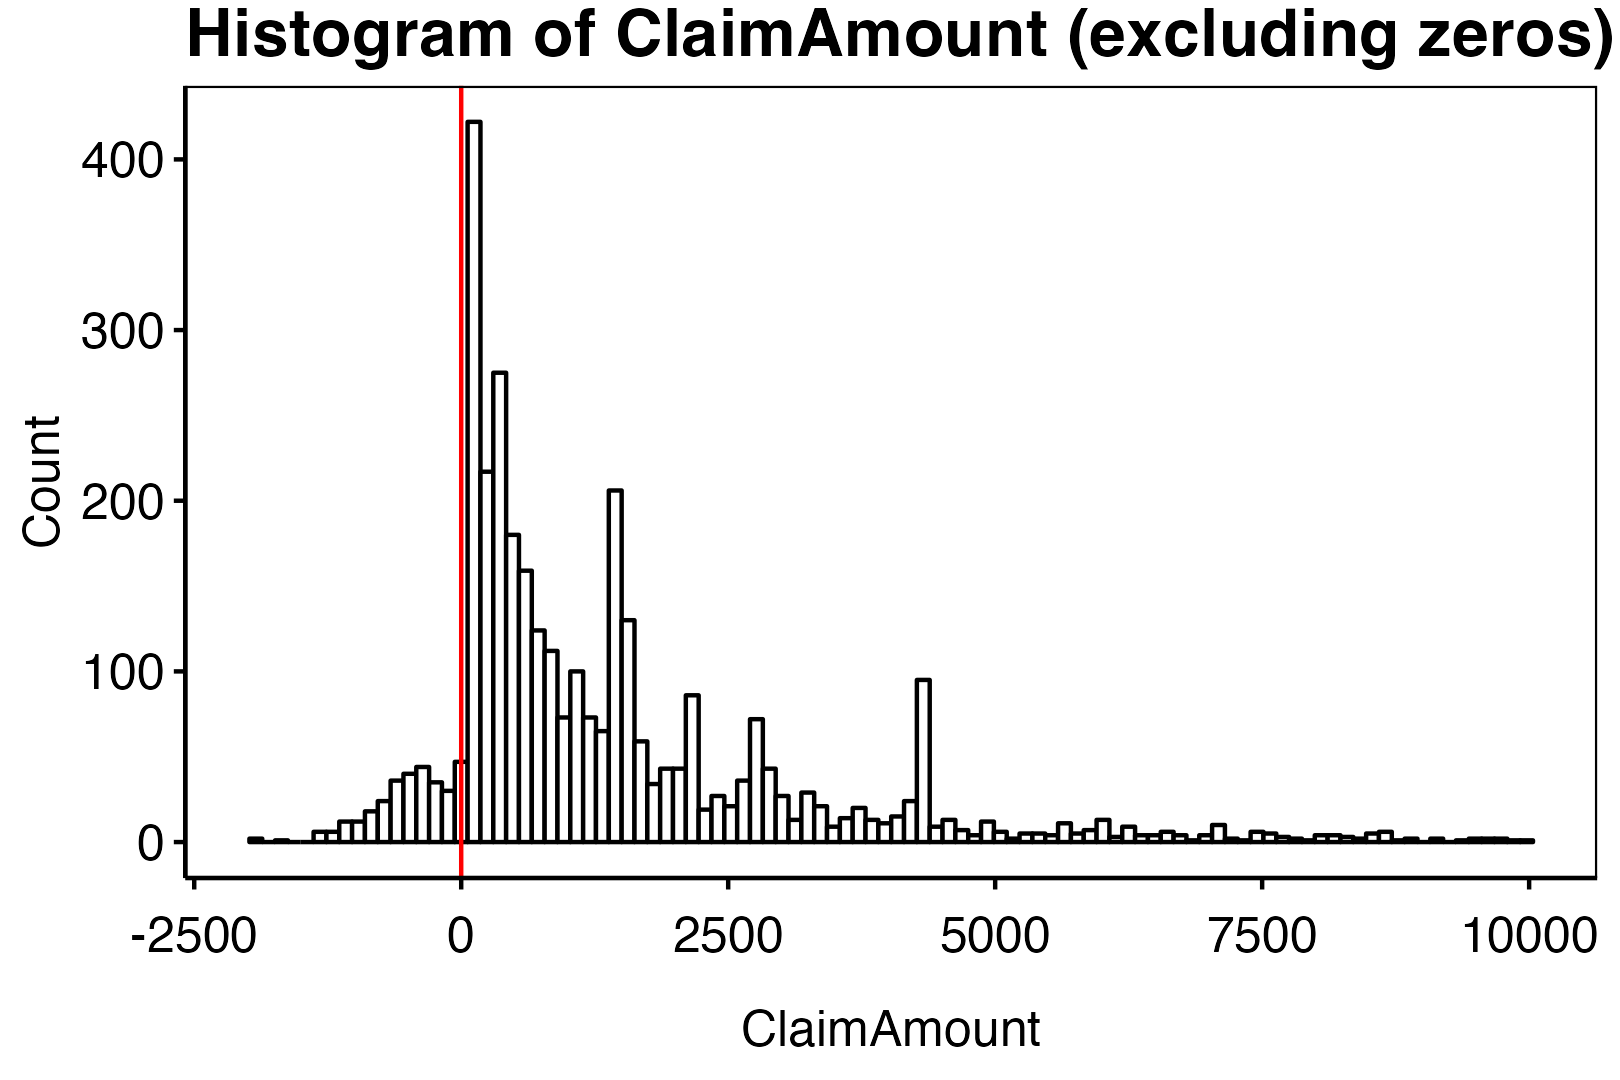
\includegraphics[width=0.48\textwidth]{figures/plot1.png}
  \end{center}
  \caption{Histogram of the variable `ClaimAmount`.}
\end{wrapfigure}

\textbf{Missing values.} As with any statistical modelling we start by
doing some exploratory analysis of the data \texttt{freMPL1}. As it was
seen in the previous section, the number of variables (columns) missing
datapoints were only one. The one in question is \texttt{RecordEnd}
which has 14143 out of 30595 missing values. This does not bather us
since we have the variable \texttt{Exposure} giving the time difference
between \texttt{RecordBeg} and \texttt{RecordEnd} in calendar years.
Furthermore we have that \texttt{RecordBeg} ranges from 2004-01-01 to
2004-12-31 and \texttt{RecordBeg\ +\ 365.25*Exposure} being at most
2004-12-31 meaning that all contracts span within the year 2004.
Assuming no seasonality trends this would incentivice us to remove the
two variables \texttt{RecordBeg} and \texttt{RecordEnd}.

\textbf{ClaimAmount and ClaimInd.} The variable of interest,
\texttt{ClaimAmount}, excibits a strange behaviour as it contains 285
strictly negative values. This is seen in figure 1. As this does not
intuitively makes sense we will set these values as zero and ensure that
the \texttt{ClaimInd} reflects this change.

\textbf{VehEngine and VehEnergy.} \emph{(Vehicle specific, 1)} Regarding
the categorical variables we notice that some levels is has sparse data.
The variables \texttt{VehEngine} and \texttt{VehEnergy} has both the
levels \texttt{GPL} and \texttt{electric}. We do however not have any
substantial datapoints as in total these levels contain 8 observations.
As the total dataset has 30595 observations in total we choose to remove
these observations.

\begin{figure}[h]
    \centering
    \subfloat[\centering]{{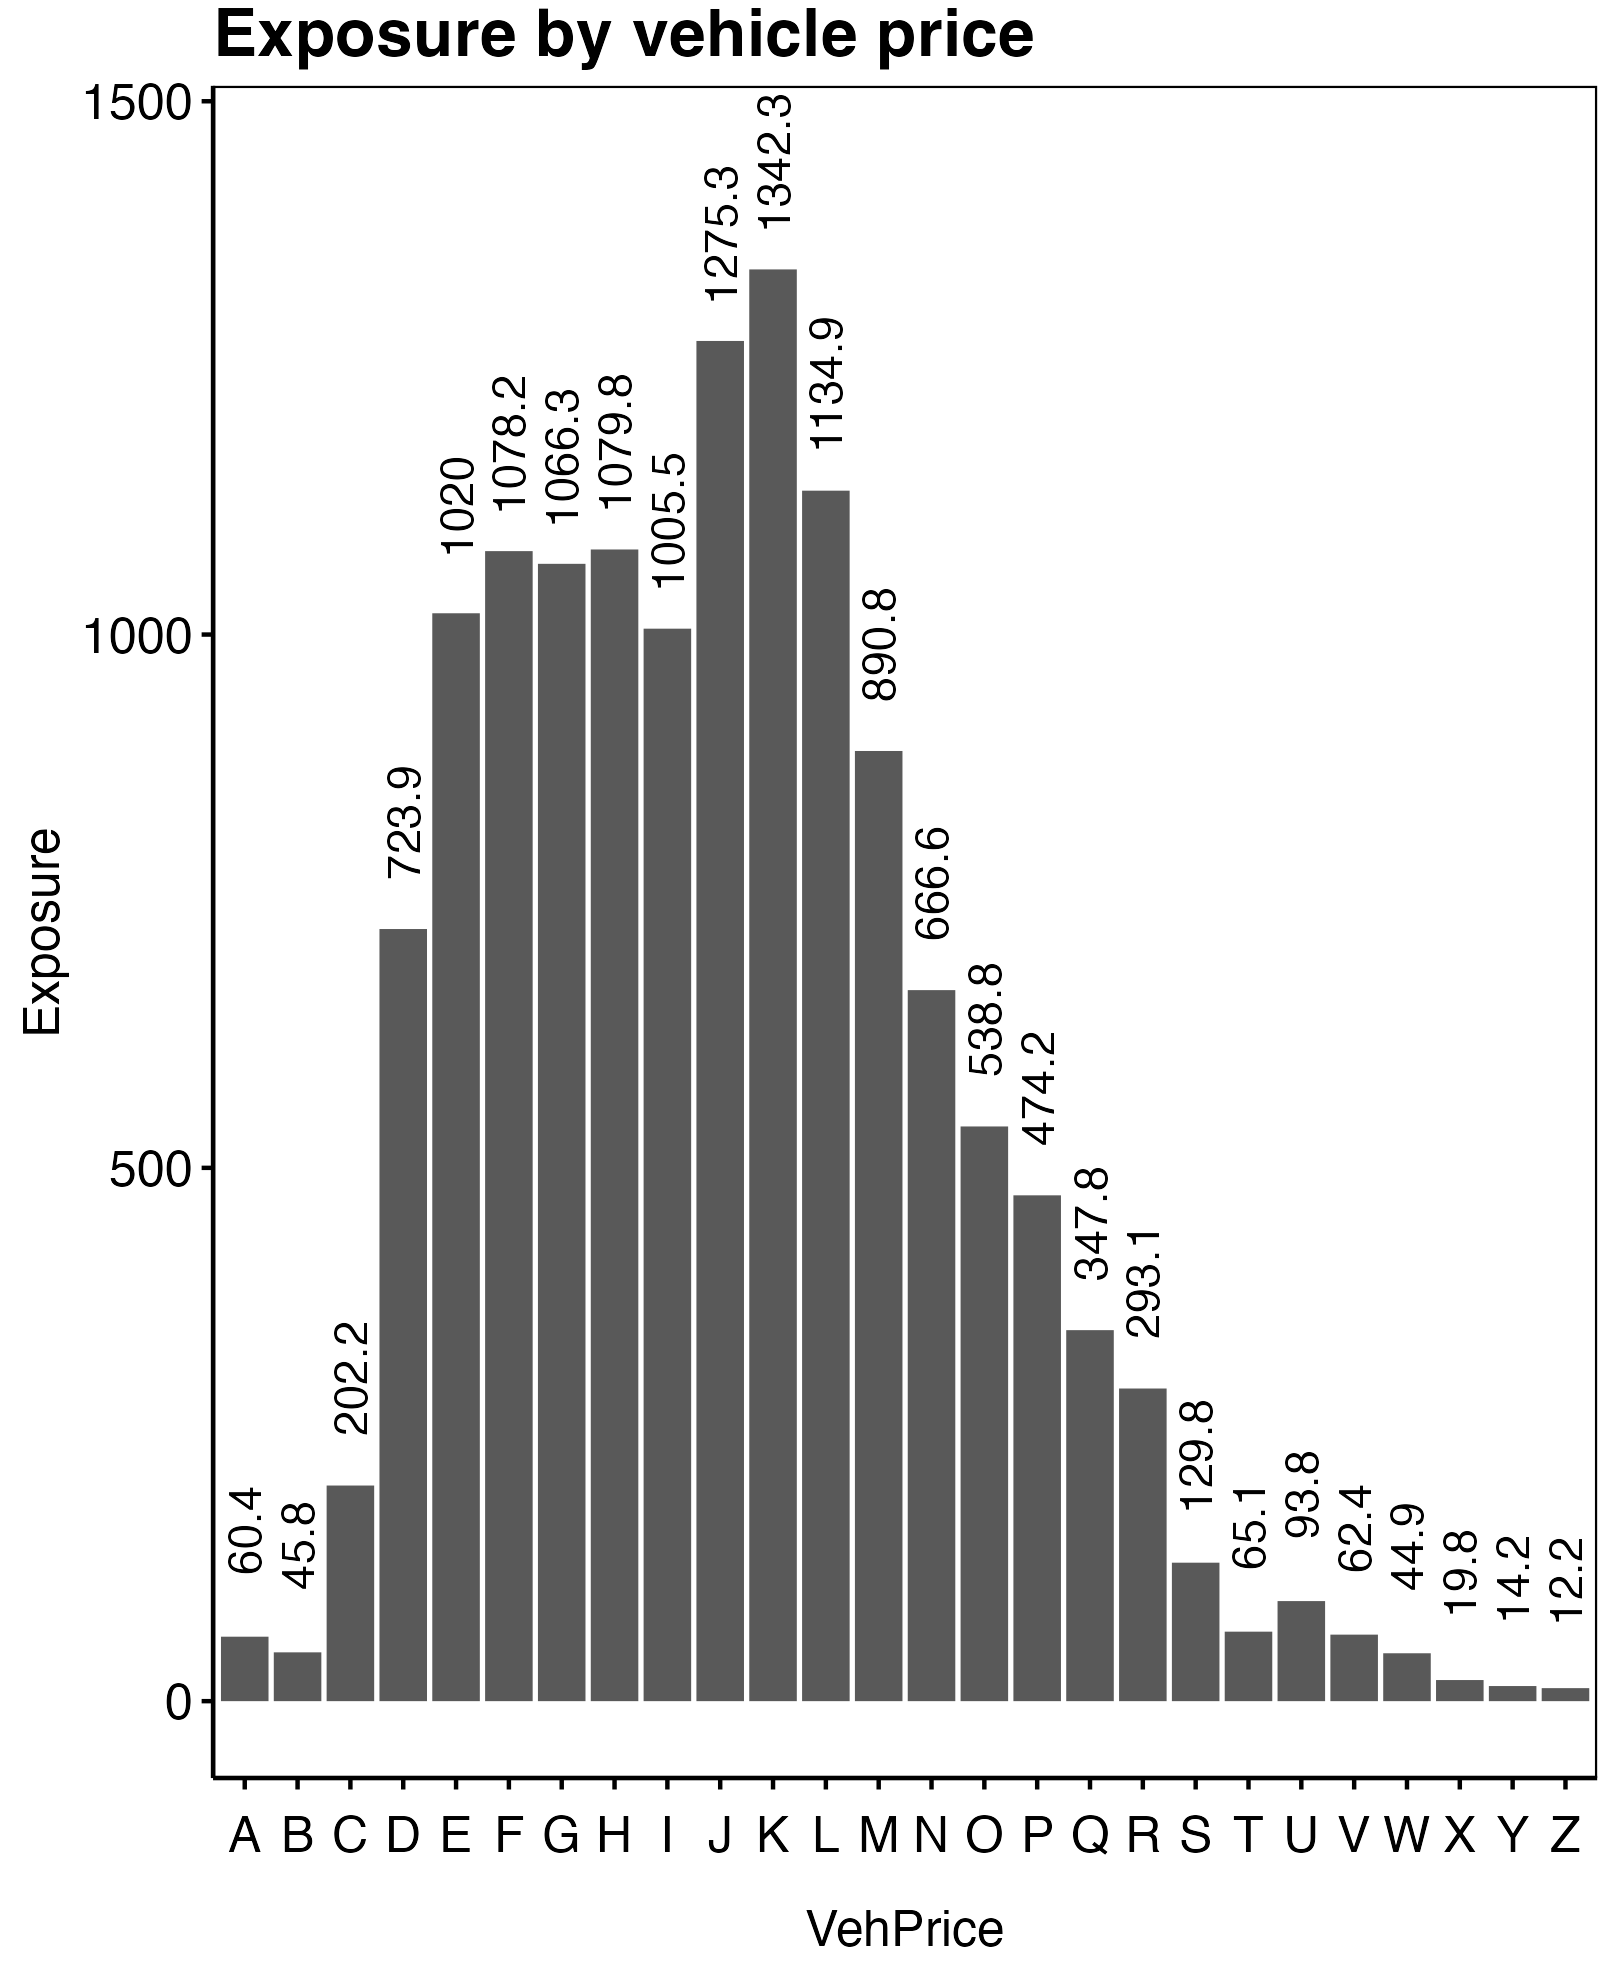
\includegraphics[width=0.25\textwidth]{figures/plot5.png} }}
    \qquad
    \subfloat[\centering]{{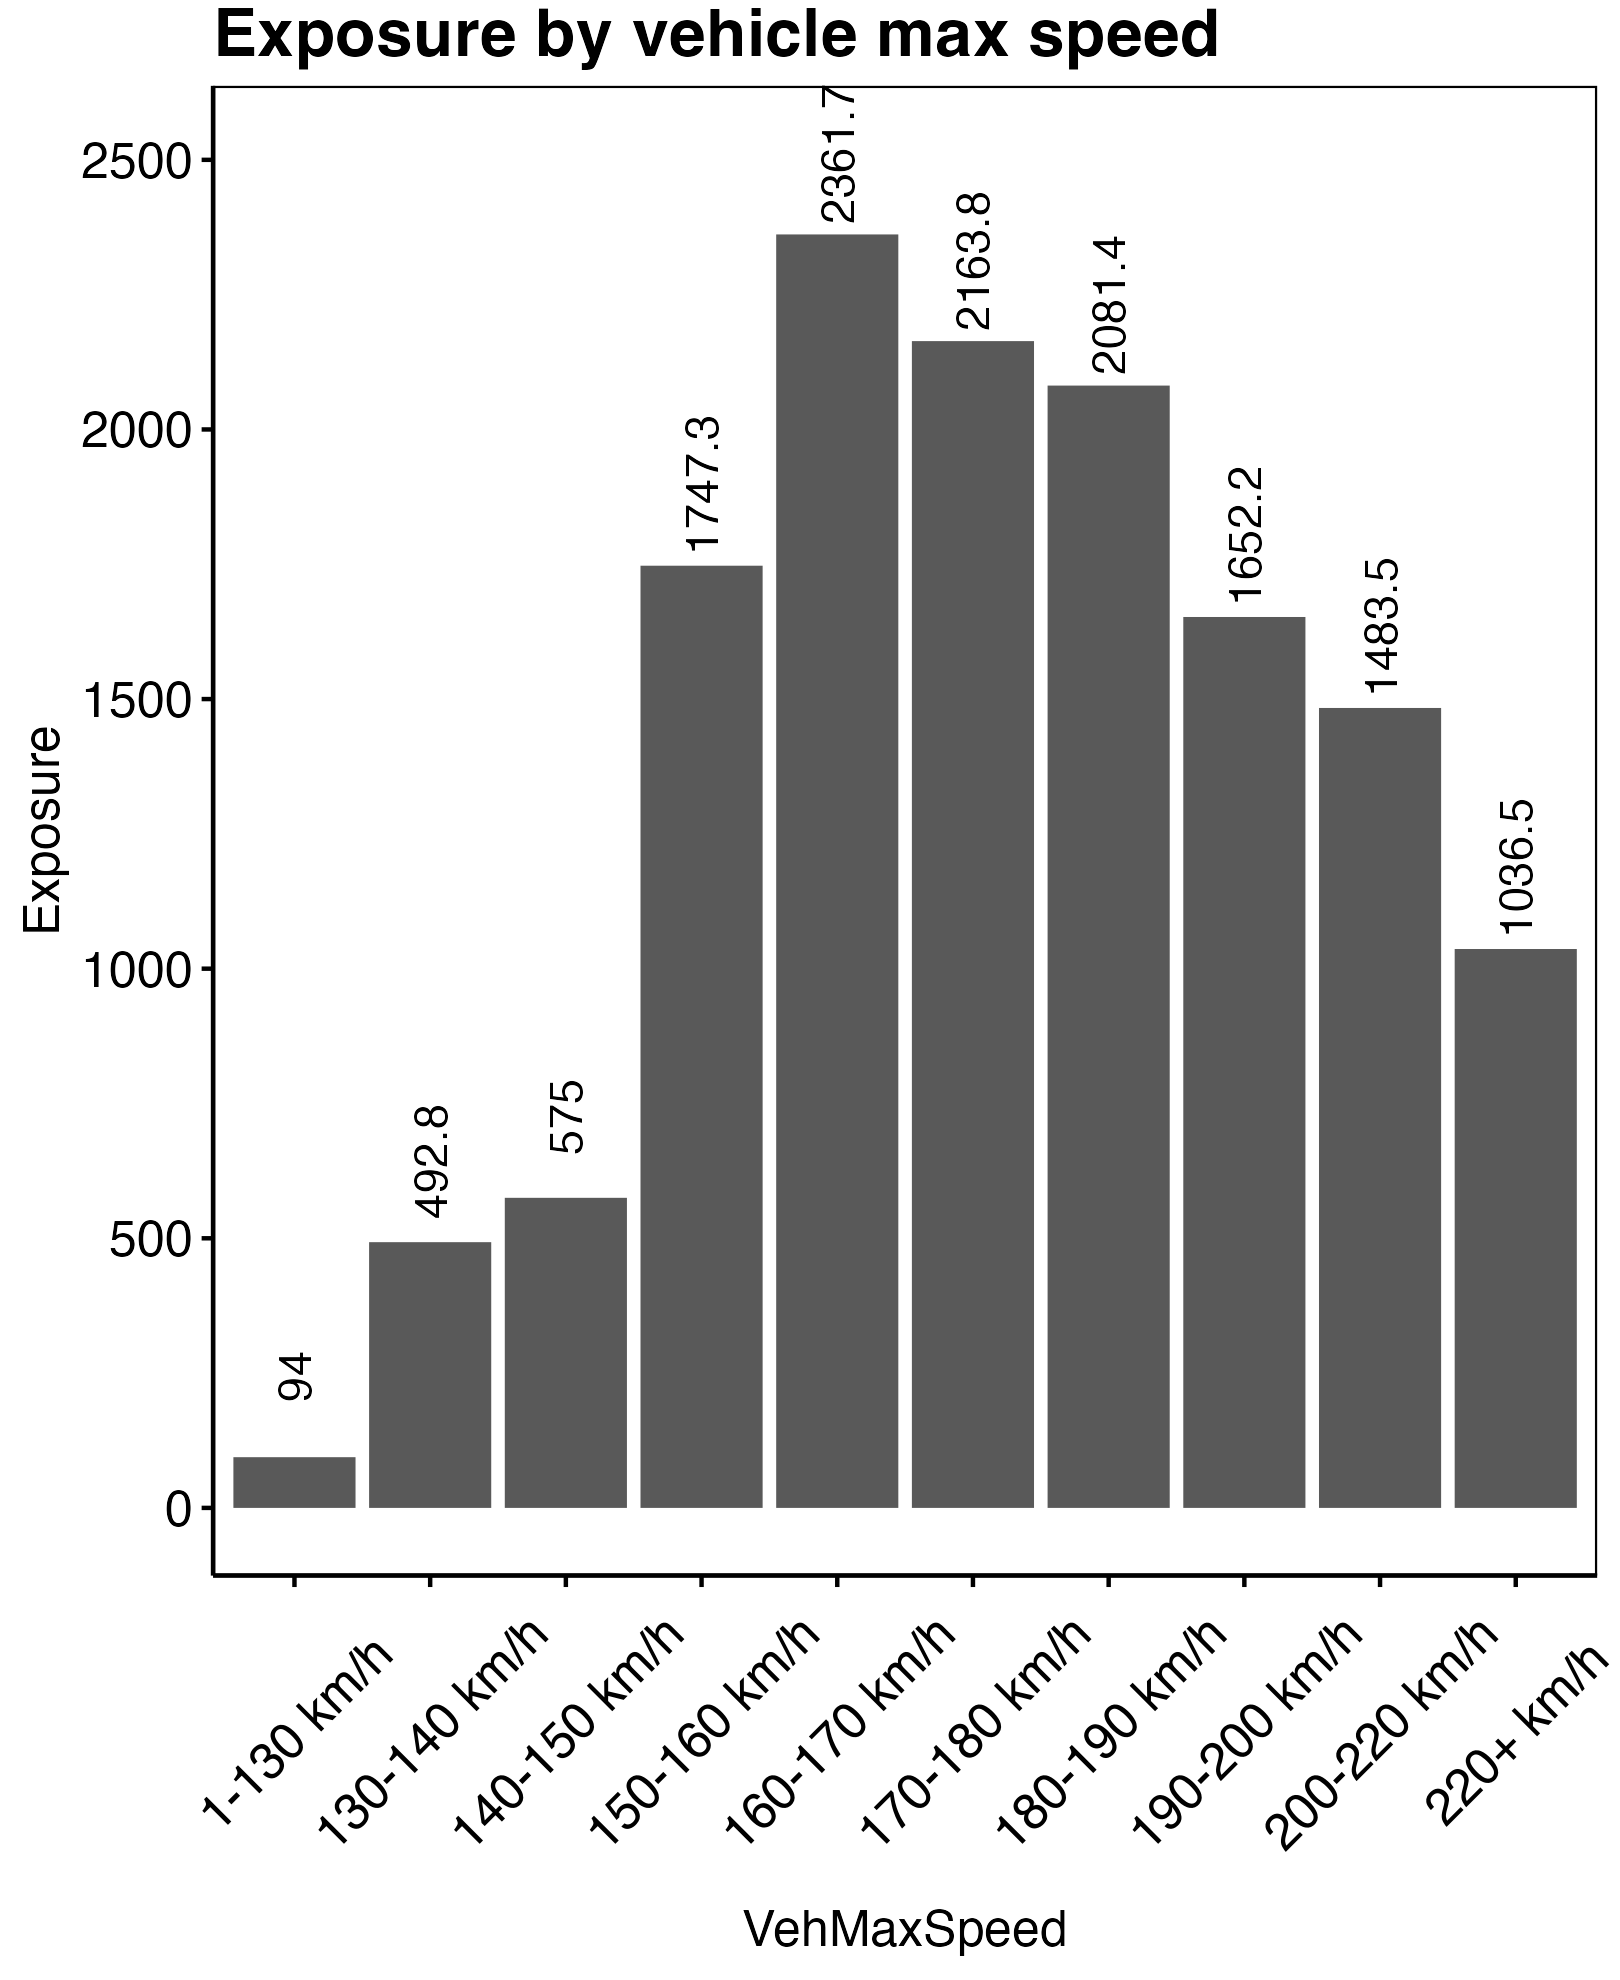
\includegraphics[width=0.25\textwidth]{figures/plot6.png} }}
    \qquad
    \subfloat[\centering]{{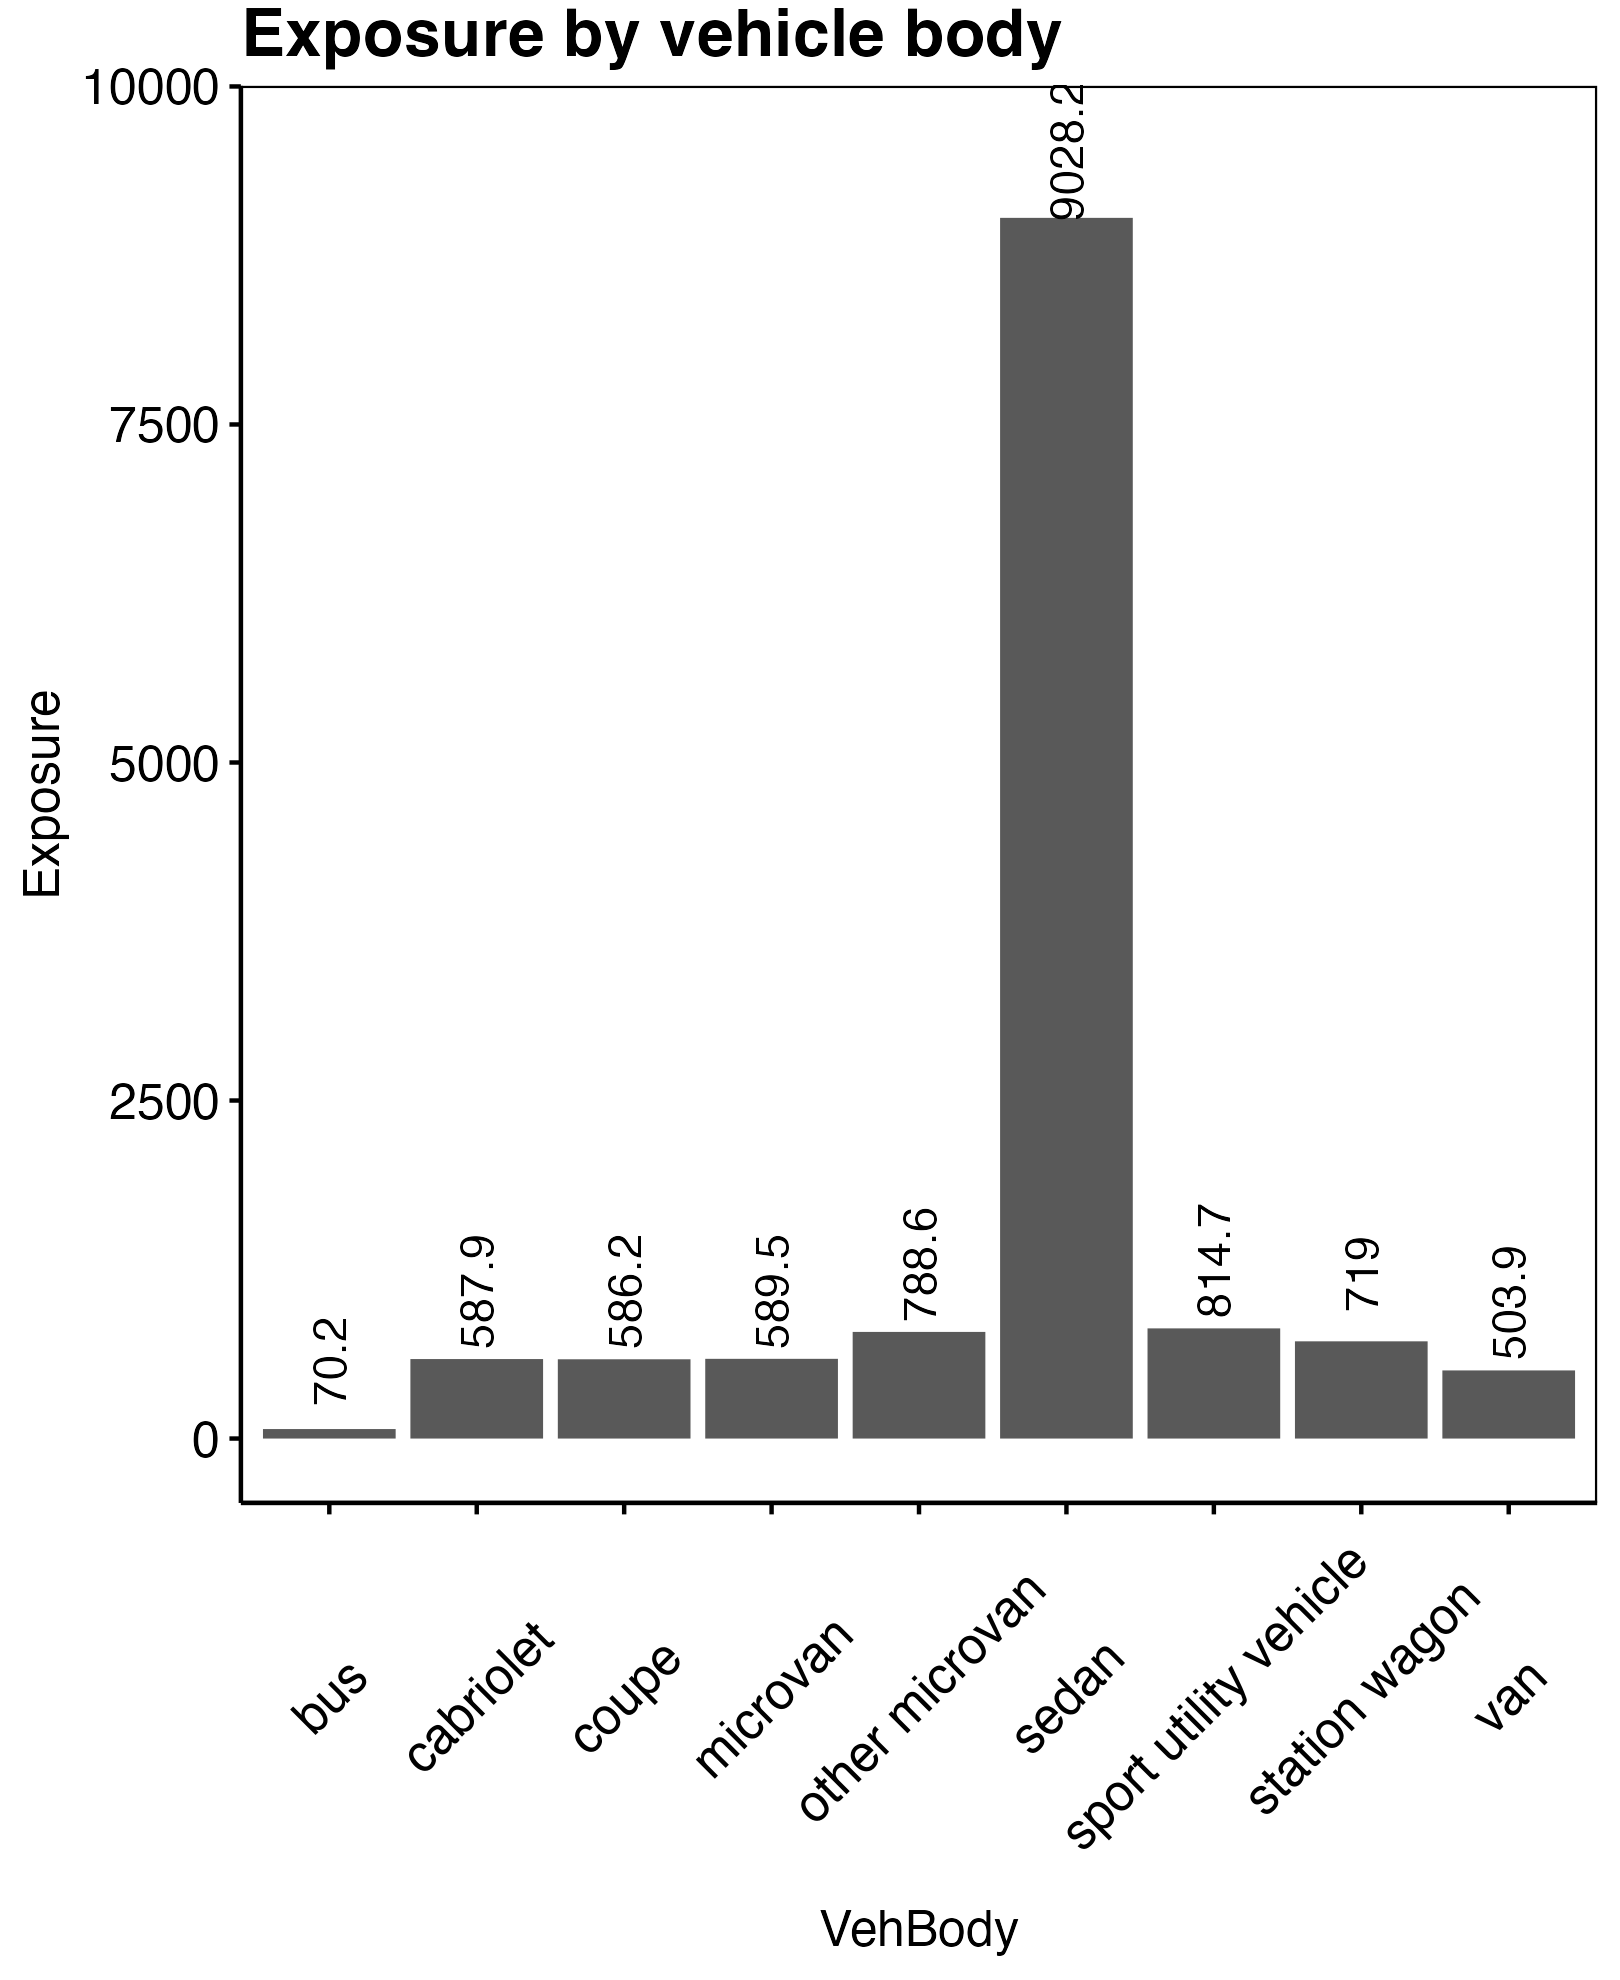
\includegraphics[width=0.25\textwidth]{figures/plot7.png} }}
    \caption{Exposure by respectively vehicle price (a), max speed (b) and body (c).}
\end{figure}

\textbf{VehPrice, VehMaxSpeed and VehBody.} \emph{(Vehicle specific, 2)}
In figure 2 we see that \texttt{VehPrice} is well represented in most
price categories. We do however har a shorter supply of data in the
tails. We will therefore combine the lowest three categories A through
C, the levels R through T and lastly U through Z. Regarding to the
vehicle max speed we see that a very few number of observations are in
the lowest category \texttt{1-130\ kmh}. We therefore combine the lowest
level with the level \texttt{130-140\ kmh}. The only vehicle body with
very few observations is \texttt{bus} with only 159 observations. We do
however see that \texttt{bus} act much like the category \texttt{sedan}
with respect to frequency and severity and so these are combined under
\texttt{sedan}.

\textbf{VehAge, VehUsage and VehClass.} \emph{(Vehicle specific, 3)} The
remaining three vehicle specific variable is well represented throughout
all levels. The only scarce observation is \texttt{VehUsage} being
\texttt{Professional\ run}. We therefore combine \texttt{Proffesional}
and \texttt{Professional\ run} under \texttt{Professional}. We leave the
remaining levels as is.

\begin{wrapfigure}{r}{0.40\textwidth}
  \begin{center}
    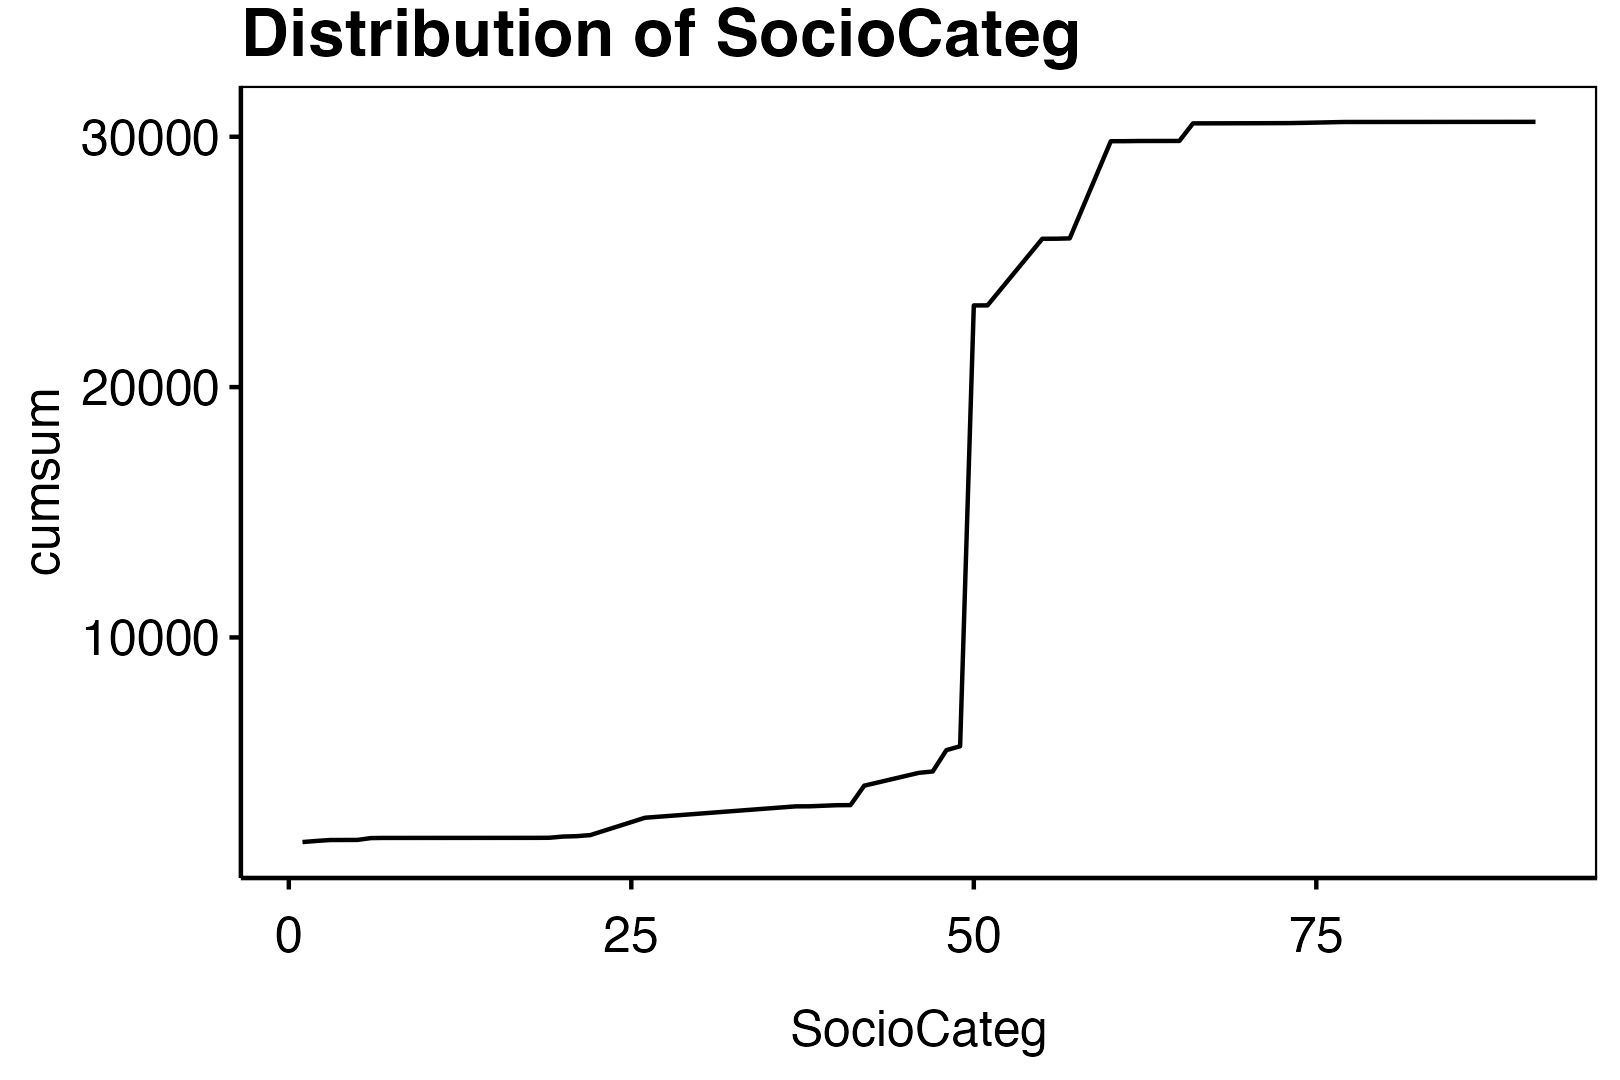
\includegraphics[width=0.38\textwidth]{figures/plot4.png}
  \end{center}
  \caption{Cummulative distribution of the variable `SocioCateg`.}
\end{wrapfigure}

\textbf{SocioCateg and Gender.} \emph{(Socails)} When constructing a
statistical model, one does not simply have to consider which variables
have the most explanatory value but one also have to take into
consideration the lawfullness of discriminating customors based on
covariates as gender, race and so forth. It is common knowledge that
insurance companies cannot discriminate based on gender and so we will
not use the variable \texttt{gender} as explanatory variable even though
it might improve the model predictions. The variable \texttt{SocioCateg}
representing the socioeconomic status of the insured ranges between
category 1 and 99. It is not at the moment clear whether this is a
covariate that may be used in pricing, so we will prefer not using it.
However, if it does indeed improve the fit without overfitting, we may
get some additional information from this variable. The data is indicate
that the custumors in general are in the category 50 with a few other
levels having significant more observations than others. For this reason
we combine the catagories from 1 to 49 into \texttt{A} and the
catagories 51 to 99 into \texttt{C} and keep the category \texttt{B} as
is.

\textbf{LicAge, DrivAge and MariStat.} \emph{(Customer specific)} In
general in France, one can acquire a drivers license at the age of 18
and so we have the obvious restriction
\texttt{LicAge\ \textless{}=\ DrivAge\ -\ 18} and we will in general
have that the license age will be approximately 18 years less than the
drivers license. It is therefore reasonable to discuss whether to
include both variables. We would however assume that for an older person
the license age would be more important than for youngsters.
Furthermore, we would assume that the \texttt{ClaimInd} and the
\texttt{LicAge} are negative correlated. We will therefore include both.
Both \texttt{Alone} and \texttt{Other} is well represented in
\texttt{MariStat}.

\textbf{HasKmLimit, RiskVar, Garage and BonusMalus} \emph{(Policy
related and others)} The variables remaining HasKmLimit, RiskVar, Garage
and BonusMalus are well represented throughout all levels and so no
action is taken here.

\begin{figure}[h]
  \begin{center}
    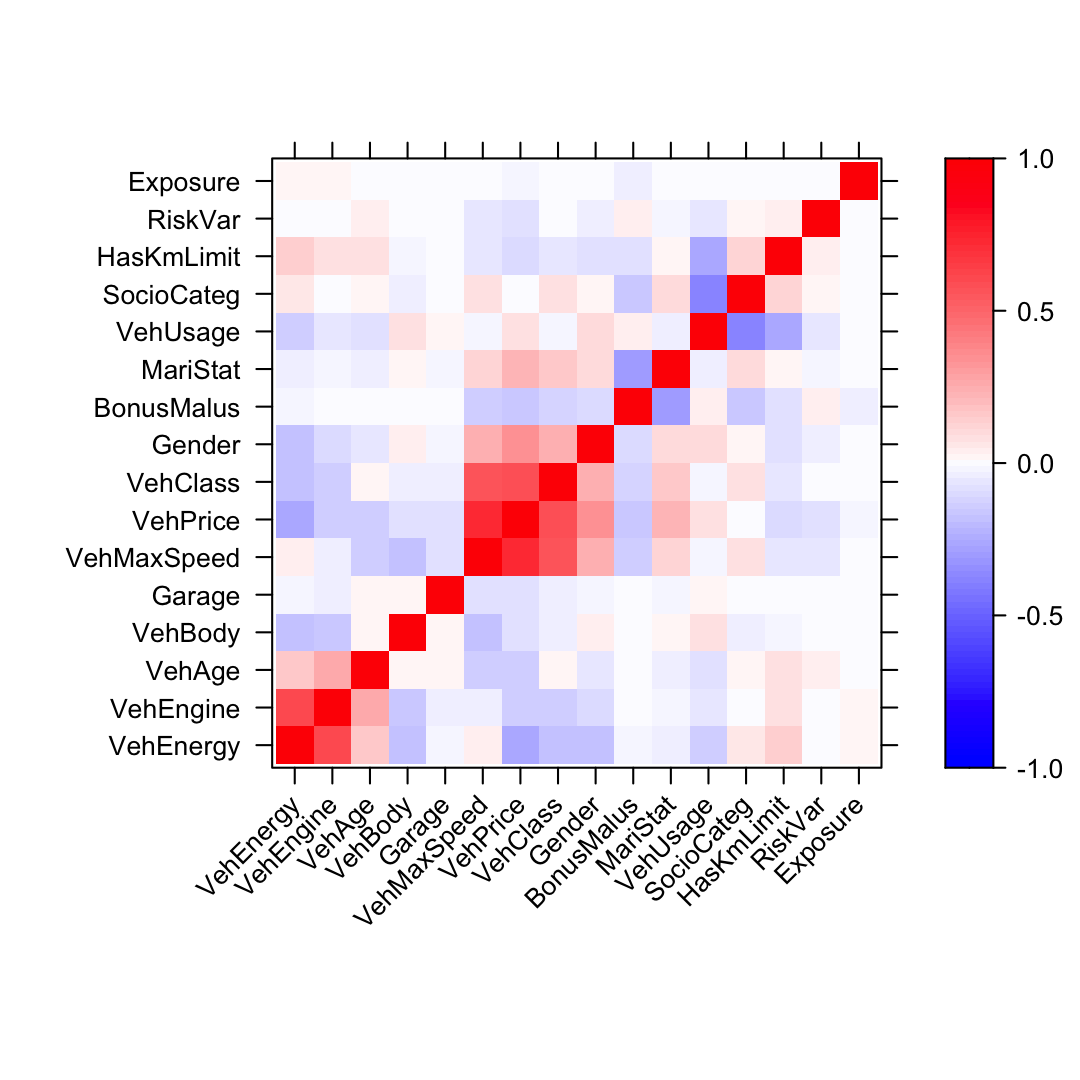
\includegraphics[width=0.48\textwidth]{figures/plot8.png}
  \end{center}
  \caption{Spearman correlation matrix.}
\end{figure}

\textbf{Correlations.} As discussed previously the age of the driver and
the license age i very correlated and so one may consider whether or not
both variables are needed. In practice we do however see that age and
experience are used when modelling the premium. Secondly, we see that
the covariates vehicle engine and energy are very correlated and also
the three variables vehicle max speed, price and class are well
correlated. Thirdly, we see that vehicle usage and socio category are
correlated. This is likely because wealthier people more often have a
car for professional use.

\newpage

\hypertarget{modelling-the-technical-premium}{%
\section{Modelling the technical
premium}\label{modelling-the-technical-premium}}

The technical premium is based upon a frequency/severity model. We have
the base model assumptions as: Let \(Y:=Y_{t+\Delta t}\) be the claim
risen by a policy during the interval \([t,t+\Delta t)\) with
\(\Delta t\) representing the exposure. Notice that in princible
\(\Delta t\) is a stopping time defined as

\[
\Delta t := \min\big(1,\inf\{s\ge t : Y_s>0\}\big),
\] meaning the policy is terminated at the time \(t+\Delta t\) with
\(t+\Delta t=t+1\) if \(Y=0\). Notice that the exposure is censored if
\(\Delta t_i<1\) and \(Y_i=0\). We furthermore have the covariates
\(X\in \mathcal X\) with \(\mathcal X\) being a \(p\)-dimensional space.
We are interested in the object \(\mathbb E[Y\ \vert\ X]\) being the
expected claim risen given the covariates \(X\). Our main assumption is
that this expectation is decomposed into

\[
\mathbb E[Y\ \vert\ X]=\mathbb E[Y1_{Y>0}\ \vert\ X]=\mathbb E[Y\ \vert\ X,1_{Y>0}]\cdot \mathbb E[1_{Y>0}\ \vert\ X]=\mu_X\cdot p_X,
\]

where \(\mu_X\) is the expected claim in the event, that a claim arises
i.e.~the severity and \(p_X\) is the probability that a claim arises
i.e.~the frequency. However since the data is censored with exposure
\(\tilde{\Delta t}\le \Delta t\) we need to consider how we may
translate a predictive model into a price function for new policies. In
practice, we include exposure as a covariate.

We will search for the most efficient estimators for both the severity
and frequency. We will denote these estimators by \(m_\mu(X)\) and
\(m_p(X)\) where we will denote the model by a superscript \(m^{(*)}_j\)
with \(*\) denoting the model for \(j=\mu,p\).

\hypertarget{severity}{%
\subsection{Severity}\label{severity}}

\begin{figure}[h]
    \centering
    \subfloat[\centering]{{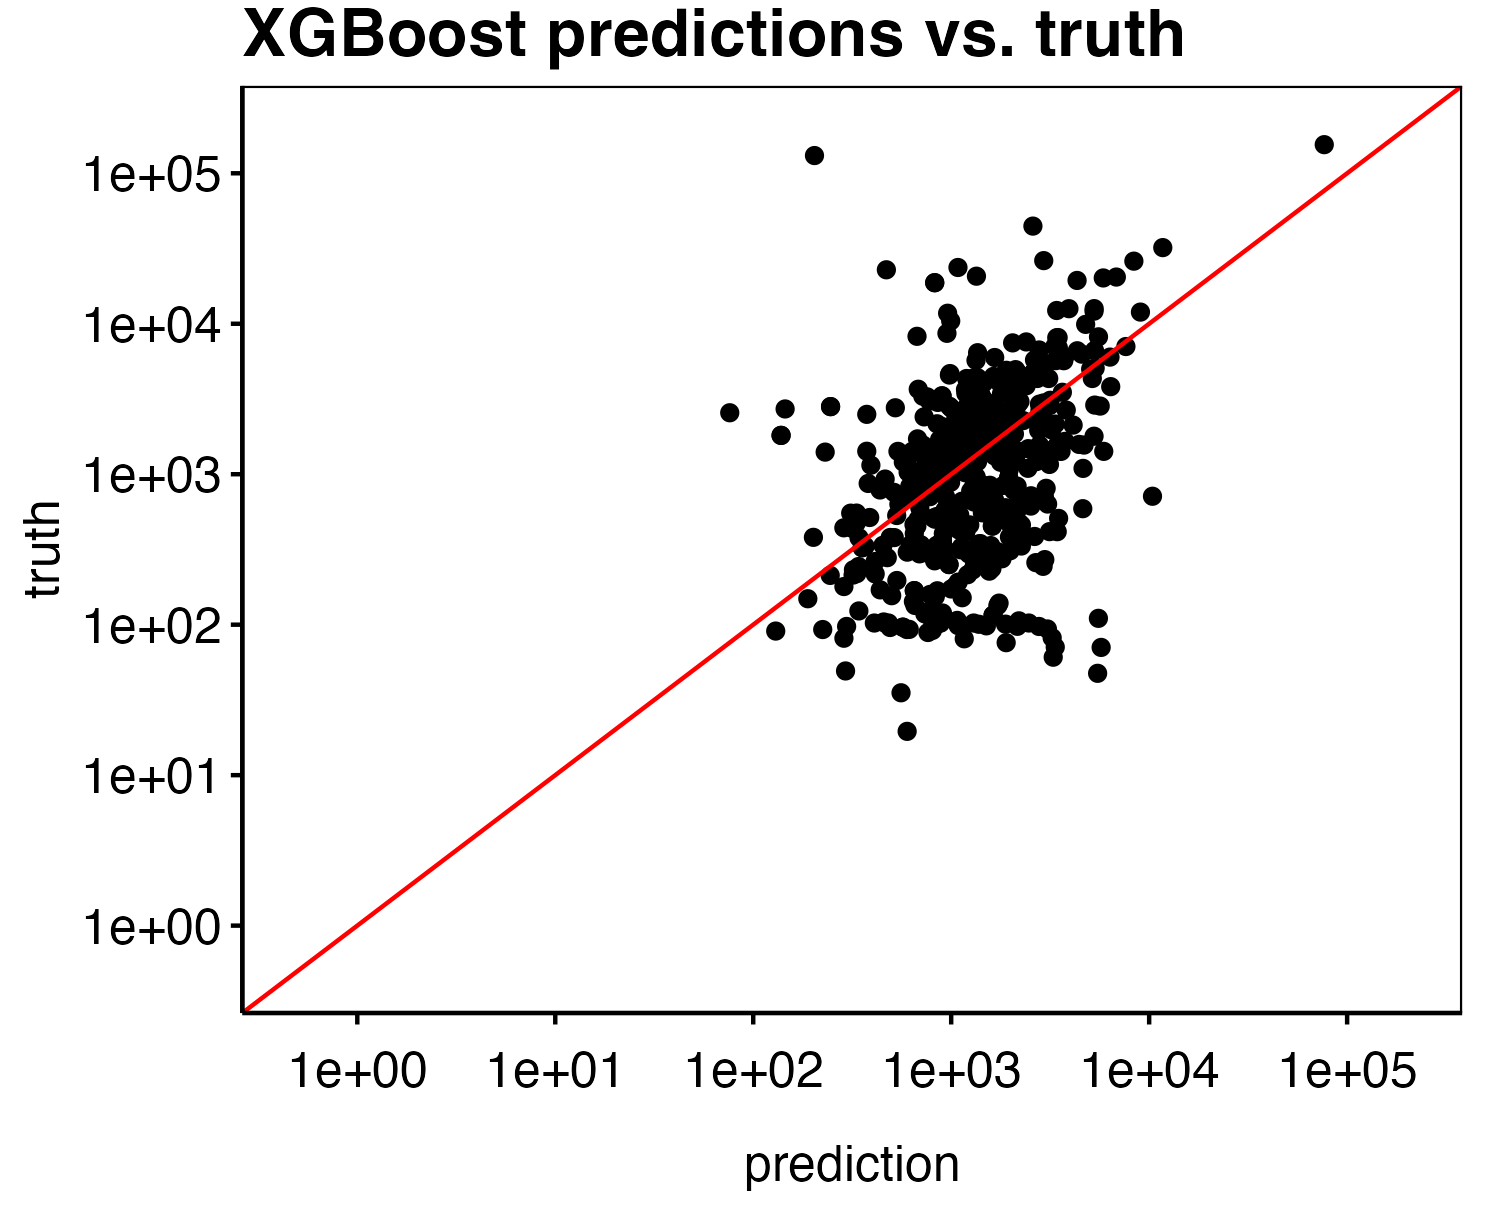
\includegraphics[width=0.45\textwidth]{figures/sev_p1.png} }}
    \qquad
    \subfloat[\centering]{{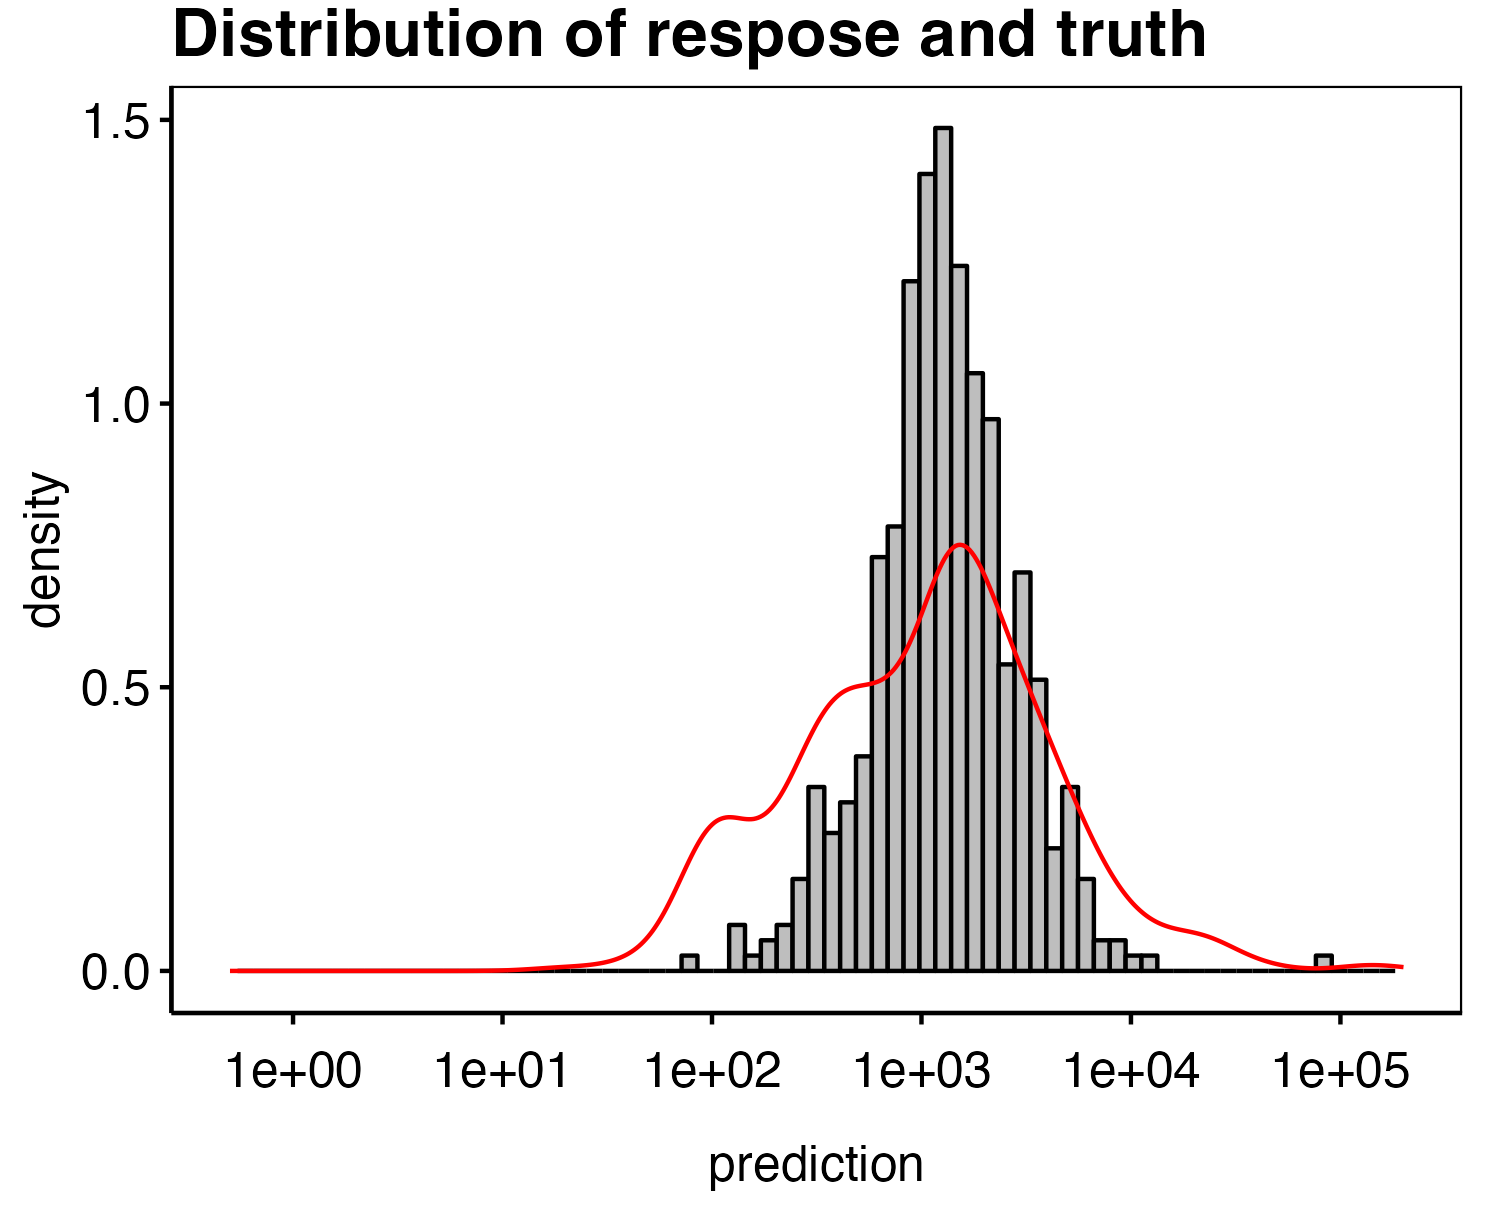
\includegraphics[width=0.45\textwidth]{figures/sev_p2.png} }}
    \caption{(a): Predictions from the model with y being the actual value and x being the estimate. The red line represent the mapping $y=x$. (b): Distribution of the response and actual values. The red density function represents the empirical density of the test data set.}
\end{figure}

We fit a XGBoost estimator to the dataset where we only consider the
non-zero claims. The distribution of the claim is rather heavy tailed as
most claims are relative small but some claims have the potential of
being large. If we fit a gamma distribution to the entire dataset, we
see that the claim amount appear to be gamma distributed with shape 0.51
and scale 4681. As such it would be appropriate to use the log link
function when fitting the parameters by setting
\texttt{objective\ =\ "reg:gamma"}. This means that the estimator
\(m_\mu(X)\) takes the form

\[
\log(\mathbb E[Y\ \vert\ X,Y>0])=m_\mu(X).
\]

Since XGBoost is a tree based algorithm with estimator
\(\hat m_\mu(X) = \sum_{i=1}^k \hat f_k(X)\) we have the decomposition

\[
\mathbb E[Y\ \vert\ X,Y>0] \approx\exp\left(\sum_{i=1}^k \hat f_k(X)\right) =\prod_{i=1}^k\exp\left(\hat f_k(X)\right),
\]

where \(k\) is the weak leaner (\texttt{nrounds}). By using the package
\texttt{mlr3} and the root mean squared loss we can estimate the
hyperparameters: leaning rate \(\eta\), depth and number og trees \(k\).
This is done using 5-fold cross validation with 1000 evals. Using the
hyperparameters the model is fitted to the dataset.

In the figure above it can be seen how the model does on the training
set using a model fitted to 85\% randomly chosen datapoints. The model
seem to predict well and we see a symmetry around \(y=x\). I does
however seem as though the estimates have less variance than the actual
claim amounts (see the (b) figure).

\hypertarget{frequency}{%
\subsection{Frequency}\label{frequency}}

\begin{wrapfigure}{r}{0.50\textwidth}
  \begin{center}
    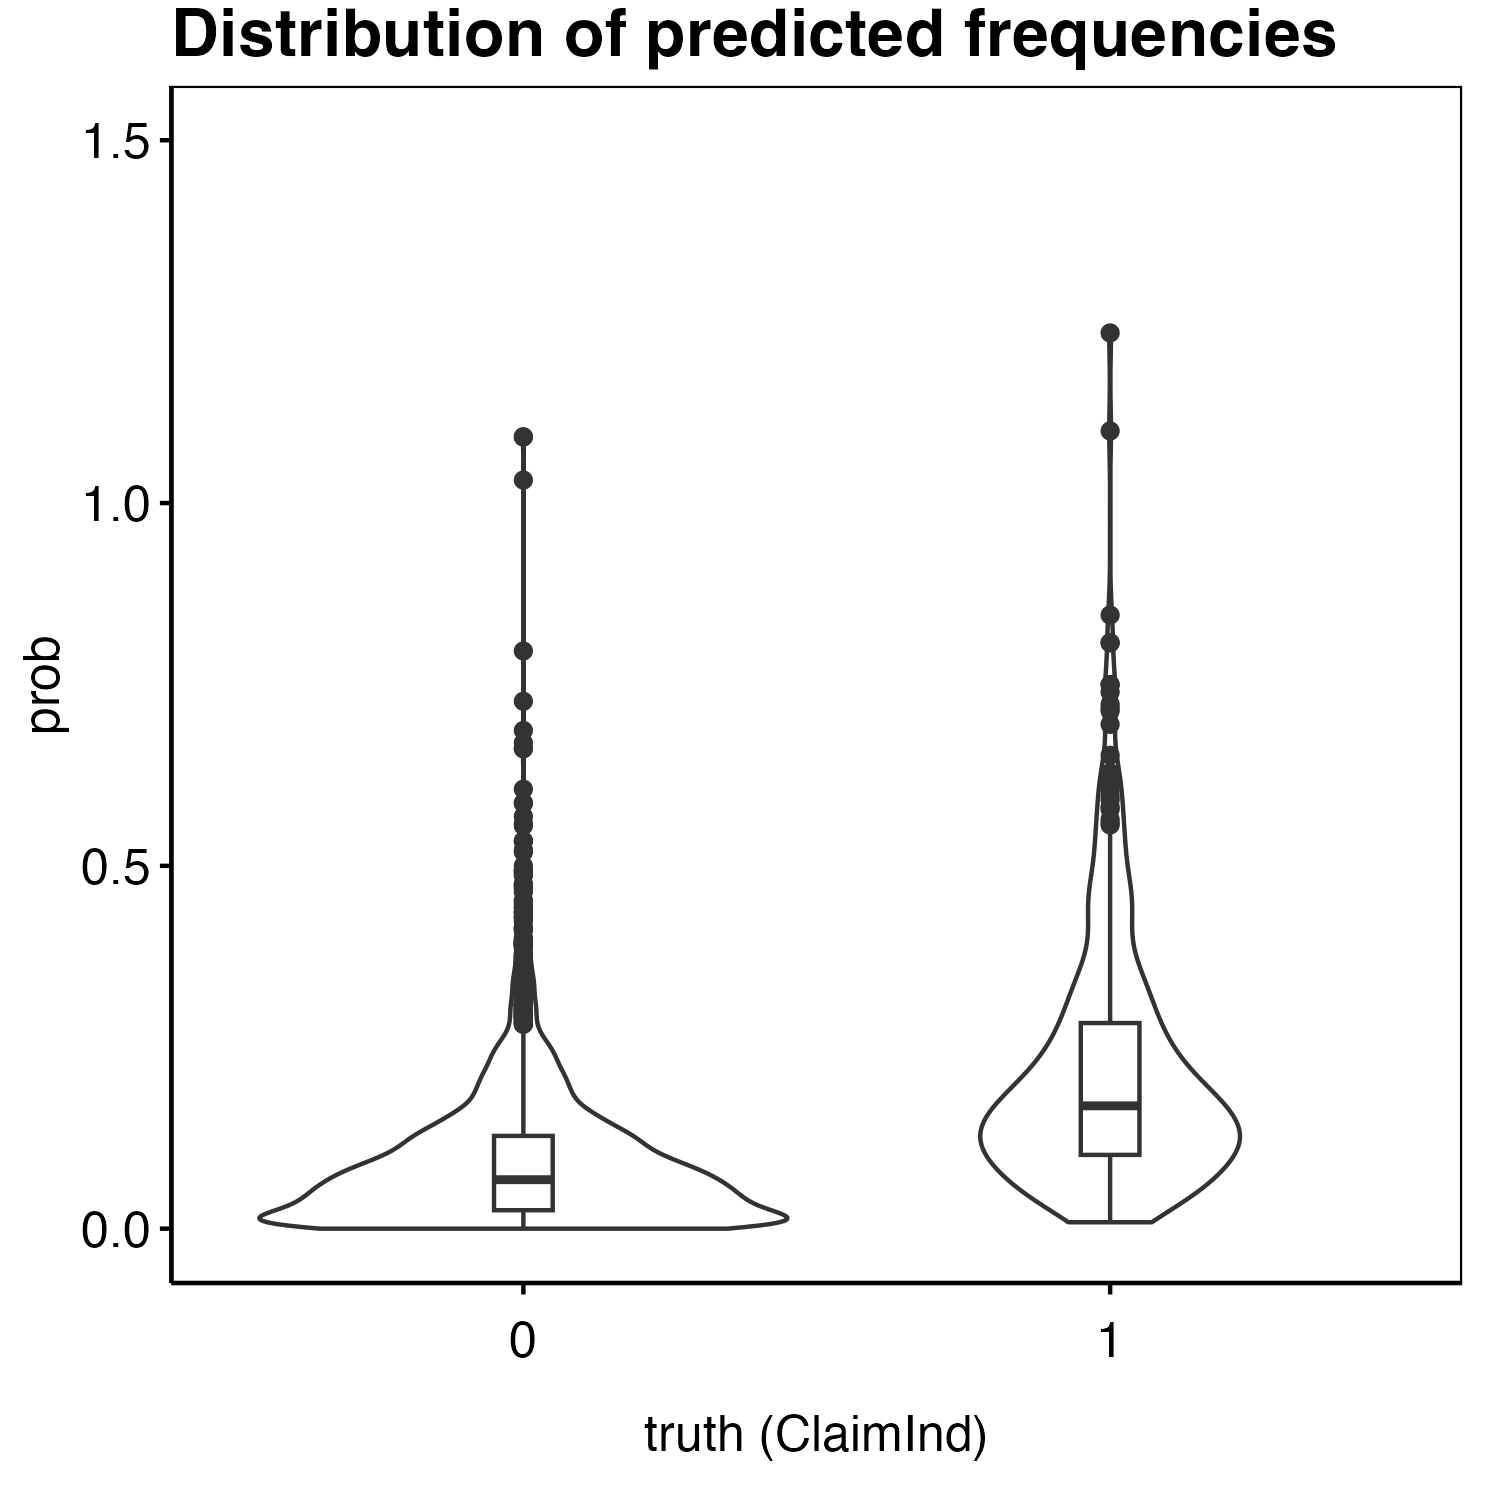
\includegraphics[width=0.48\textwidth]{figures/freq_p1.png}
  \end{center}
  \caption{A combined boxplot and violin plot of the distribution of the predicted probability for respectively the non claim (left) and claim (right) policies.}
\end{wrapfigure}

The frequency is modeled using the \texttt{xgboost} packages. The claims
is assumed to arrive poisson distributed given the covariates \(X\) and
so the XGBoost estimator is fitted with
\texttt{objective\ =\ "count:poisson"}. This implements the log-link
function and optimizes using the gradient of the poisson deviance.

Like in the case of the severity model we have the same log link
function and so for trees \(1,...,l\) we will have the estimate

\[
\mathbb E[1_{Y>0}\ \vert\ X]\approx\prod_{i=1}^l\exp(g_i(X)).
\]

In the figure on the right, we see that the algorithm fit higher
probabilities (frequencies) to policies that actually happened to raise
a claim.

\hypertarget{initial-estimate-of-the-technical-premium}{%
\subsection{Initial estimate of the technical
premium}\label{initial-estimate-of-the-technical-premium}}

The technical price is given by the product

\[
\pi=\mu_X\cdot p_X.
\]

Notice that the length of the contract i.e.~the exposure is used as a
covariate in the frequency/severity model, and so the effect of longer
contracts is already priced in. By default new contracts are sold with a
yearly length, however in the case of estimating on the dataset we use
the given \texttt{Exposure}. Up untill now we have used the protected
feature gender in the estimate, so we start by fitting a biased estimate

\[
\hat \pi^{(biased)}=\hat m_\mu^{(biased)}(X)\cdot\hat m_p^{(biased)}(X).
\]

We can apply the technical price onto the dataset \texttt{df} by running
the following code:

\begin{Shaded}
\begin{Highlighting}[]
\CommentTok{\# Estimating mu}
\NormalTok{sev\_covariates }\OtherTok{\textless{}{-}}\NormalTok{ df[,sev\_columns] }\SpecialCharTok{\%\textgreater{}\%}
  \FunctionTok{select}\NormalTok{(}\SpecialCharTok{{-}}\NormalTok{ClaimInd,}\SpecialCharTok{{-}}\NormalTok{ID,}\SpecialCharTok{{-}}\NormalTok{ClaimAmount,}\SpecialCharTok{{-}}\NormalTok{Exposure)}
\NormalTok{sev\_covariates }\OtherTok{\textless{}{-}}  \FunctionTok{as.matrix}\NormalTok{(sev\_covariates)}
\NormalTok{m\_mu }\OtherTok{\textless{}{-}} \FunctionTok{predict}\NormalTok{(xgb\_regr, }\AttributeTok{newdata =}\NormalTok{ sev\_covariates)}
\CommentTok{\# Estimating p}
\NormalTok{freq\_covariates }\OtherTok{\textless{}{-}}\NormalTok{ df[,freq\_columns] }\SpecialCharTok{\%\textgreater{}\%}
  \FunctionTok{select}\NormalTok{(}\SpecialCharTok{{-}}\NormalTok{ClaimInd,}\SpecialCharTok{{-}}\NormalTok{ID,}\SpecialCharTok{{-}}\NormalTok{ClaimAmount)}
\NormalTok{freq\_covariates }\OtherTok{\textless{}{-}} \FunctionTok{as.matrix}\NormalTok{(freq\_covariates)}
\NormalTok{m\_p }\OtherTok{\textless{}{-}} \FunctionTok{predict}\NormalTok{(xgb\_freq\_train, }\AttributeTok{newdata =}\NormalTok{ freq\_covariates)}
\NormalTok{freq\_covariates[,}\StringTok{"Exposure"}\NormalTok{] }\OtherTok{\textless{}{-}} \DecValTok{1}
\NormalTok{m\_p\_2 }\OtherTok{\textless{}{-}} \FunctionTok{predict}\NormalTok{(xgb\_freq\_train, }\AttributeTok{newdata =}\NormalTok{ freq\_covariates)}
\CommentTok{\# Inserting estimates}
\NormalTok{df[,}\StringTok{"pi\_hat"}\NormalTok{] }\OtherTok{\textless{}{-}}\NormalTok{ m\_mu }\SpecialCharTok{*}\NormalTok{ m\_p}
\NormalTok{df[,}\StringTok{"mu\_hat"}\NormalTok{] }\OtherTok{\textless{}{-}}\NormalTok{ m\_mu}
\NormalTok{df[,}\StringTok{"p\_hat"}\NormalTok{] }\OtherTok{\textless{}{-}}\NormalTok{ m\_p}
\NormalTok{df[,}\StringTok{"p\_hat\_new"}\NormalTok{] }\OtherTok{\textless{}{-}}\NormalTok{ m\_p\_2}
\NormalTok{df[,}\StringTok{"pi\_hat\_new"}\NormalTok{] }\OtherTok{\textless{}{-}}\NormalTok{ m\_mu }\SpecialCharTok{*}\NormalTok{ m\_p\_2}
\end{Highlighting}
\end{Shaded}

We can summarize the models predictions on the policies below.

\begin{longtable}[t]{llllllllll}
\caption{\label{tab:unnamed-chunk-7}Comparing premiums}\\
\toprule
\multicolumn{2}{c}{ } & \multicolumn{4}{c}{Actual} & \multicolumn{4}{c}{Extrapolated} \\
\cmidrule(l{3pt}r{3pt}){3-6} \cmidrule(l{3pt}r{3pt}){7-10}
Policy & Gender & Exposure & p(Y>0) & E(Y|Y>0) & Price & Exposure & p(Y>0) & E(Y|Y>0) & Price\\
\midrule
\endfirsthead
\caption[]{Comparing premiums \textit{(continued)}}\\
\toprule
\multicolumn{2}{c}{ } & \multicolumn{4}{c}{Actual} & \multicolumn{4}{c}{Extrapolated} \\
\cmidrule(l{3pt}r{3pt}){3-6} \cmidrule(l{3pt}r{3pt}){7-10}
Policy & Gender & Exposure & p(Y>0) & E(Y|Y>0) & Price & Exposure & p(Y>0) & E(Y|Y>0) & Price\\
\midrule
\endhead

\endfoot
\bottomrule
\endlastfoot
\cellcolor{gray!6}{6254} & \cellcolor{gray!6}{Female} & \cellcolor{gray!6}{0.083} & \cellcolor{gray!6}{0.0465} & \cellcolor{gray!6}{1051} & \cellcolor{gray!6}{48.9} & \cellcolor{gray!6}{1} & \cellcolor{gray!6}{0.154} & \cellcolor{gray!6}{1051} & \cellcolor{gray!6}{161.5}\\
24123 & Male & 0.633 & 0.1677 & 917 & 153.7 & 1 & 0.191 & 917 & 175.1\\
\cellcolor{gray!6}{25010} & \cellcolor{gray!6}{Female} & \cellcolor{gray!6}{0.208} & \cellcolor{gray!6}{0.1097} & \cellcolor{gray!6}{1226} & \cellcolor{gray!6}{134.4} & \cellcolor{gray!6}{1} & \cellcolor{gray!6}{0.499} & \cellcolor{gray!6}{1226} & \cellcolor{gray!6}{611.8}\\
25188 & Male & 0.095 & 0.0524 & 2468 & 129.4 & 1 & 0.223 & 2468 & 550.8\\
\cellcolor{gray!6}{30495} & \cellcolor{gray!6}{Female} & \cellcolor{gray!6}{0.751} & \cellcolor{gray!6}{0.1034} & \cellcolor{gray!6}{755} & \cellcolor{gray!6}{78.1} & \cellcolor{gray!6}{1} & \cellcolor{gray!6}{0.113} & \cellcolor{gray!6}{755} & \cellcolor{gray!6}{85.5}\\
\addlinespace
30555 & Male & 0.163 & 0.0338 & 617 & 20.9 & 1 & 0.145 & 617 & 89.6\\*
\end{longtable}

In the table above we have altered the dataset with exposure set to 1
for all rows, to predict the price of a new contract i.e.~with exposure
of one year. One sees that the prices for the new contracts are larger
than the technical price for the historical as the exposure is larger.
Furthermore as expected we see that the estimate \(\hat \mu_X\) does not
depend on the exposure.

\newpage

\hypertarget{decomposing-the-estimates}{%
\section{Decomposing the estimates}\label{decomposing-the-estimates}}

\newpage

\hypertarget{discrimination-and-debaissing-of-the-model}{%
\section{Discrimination and debaissing of the
model}\label{discrimination-and-debaissing-of-the-model}}

\begin{longtable}[t]{llllllll}
\caption{\label{tab:unnamed-chunk-11}Comparing premiums}\\
\toprule
\multicolumn{2}{c}{ } & \multicolumn{3}{c}{Biased} & \multicolumn{3}{c}{Debiased} \\
\cmidrule(l{3pt}r{3pt}){3-5} \cmidrule(l{3pt}r{3pt}){6-8}
Policy & Gender & p(Y>0) & E(Y|Y>0) & Price & p(Y>0) & E(Y|Y>0) & Price\\
\midrule
\endfirsthead
\caption[]{Comparing premiums \textit{(continued)}}\\
\toprule
\multicolumn{2}{c}{ } & \multicolumn{3}{c}{Biased} & \multicolumn{3}{c}{Debiased} \\
\cmidrule(l{3pt}r{3pt}){3-5} \cmidrule(l{3pt}r{3pt}){6-8}
Policy & Gender & p(Y>0) & E(Y|Y>0) & Price & p(Y>0) & E(Y|Y>0) & Price\\
\midrule
\endhead

\endfoot
\bottomrule
\endlastfoot
\cellcolor{gray!6}{6254} & \cellcolor{gray!6}{Female} & \cellcolor{gray!6}{0.0465} & \cellcolor{gray!6}{1051} & \cellcolor{gray!6}{48.9} & \cellcolor{gray!6}{0.0550} & \cellcolor{gray!6}{1007} & \cellcolor{gray!6}{55.4}\\
24123 & Male & 0.1677 & 917 & 153.7 & 0.1469 & 932 & 136.9\\
\cellcolor{gray!6}{25010} & \cellcolor{gray!6}{Female} & \cellcolor{gray!6}{0.1097} & \cellcolor{gray!6}{1226} & \cellcolor{gray!6}{134.4} & \cellcolor{gray!6}{0.1074} & \cellcolor{gray!6}{1189} & \cellcolor{gray!6}{127.7}\\
25188 & Male & 0.0524 & 2468 & 129.4 & 0.0502 & 2518 & 126.4\\
\cellcolor{gray!6}{30495} & \cellcolor{gray!6}{Female} & \cellcolor{gray!6}{0.1034} & \cellcolor{gray!6}{755} & \cellcolor{gray!6}{78.1} & \cellcolor{gray!6}{0.0976} & \cellcolor{gray!6}{804} & \cellcolor{gray!6}{78.4}\\
\addlinespace
30555 & Male & 0.0338 & 617 & 20.9 & 0.0296 & 618 & 18.3\\*
\end{longtable}

\newpage

\hypertarget{repreducing-statement}{%
\section{Repreducing statement}\label{repreducing-statement}}

\hypertarget{packages}{%
\subsection{Packages}\label{packages}}

\begin{Shaded}
\begin{Highlighting}[]
\FunctionTok{library}\NormalTok{(CASdatasets)}
\FunctionTok{library}\NormalTok{(lattice)}
\FunctionTok{library}\NormalTok{(evmix)}
\FunctionTok{library}\NormalTok{(ggplot2)}
\FunctionTok{library}\NormalTok{(mlr3)}
\FunctionTok{library}\NormalTok{(mlr3learners)}
\FunctionTok{library}\NormalTok{(mlr3extralearners)}
\FunctionTok{library}\NormalTok{(dbarts)}
\FunctionTok{library}\NormalTok{(mlr3mbo)}
\FunctionTok{library}\NormalTok{(mlr3measures)}
\FunctionTok{library}\NormalTok{(mlr3tuning)}
\FunctionTok{library}\NormalTok{(ranger)}
\FunctionTok{library}\NormalTok{(mlr3viz)}
\FunctionTok{library}\NormalTok{(fastDummies)}
\FunctionTok{library}\NormalTok{(dplyr)}
\FunctionTok{library}\NormalTok{(patchwork)}
\FunctionTok{library}\NormalTok{(xgboost)}
\FunctionTok{library}\NormalTok{(glex)}
\FunctionTok{library}\NormalTok{(treeshap)}
\end{Highlighting}
\end{Shaded}

\hypertarget{statistical-data}{%
\subsection{Statistical data}\label{statistical-data}}

The data we will be working with is the \texttt{freMPL1} (\emph{French
Motor Personal Line datasets}) dataset from the package
\texttt{CASdatasets} (\emph{Computational Actuarial Science datasets}).
The author write the following regarding the dataset

\begin{quote}
This collection of ten datasets comes from a private motor French
insurer. Each dataset includes risk features, claim amount and claim
history of around 30,000 policies for year 2004.
\end{quote}

A detailed description of the variables may be read in the below table.

\begin{longtable}[]{@{}
  >{\raggedright\arraybackslash}p{(\columnwidth - 2\tabcolsep) * \real{0.4211}}
  >{\raggedright\arraybackslash}p{(\columnwidth - 2\tabcolsep) * \real{0.5789}}@{}}
\toprule()
\begin{minipage}[b]{\linewidth}\raggedright
Variable
\end{minipage} & \begin{minipage}[b]{\linewidth}\raggedright
Description
\end{minipage} \\
\midrule()
\endhead
\emph{Exposure} & The exposure, in years. \\
\emph{LicAge} & The driving licence age, in months. \\
\emph{RecordBeg} & Beginning date of record. \\
\emph{RecordEnd} & End date of record. \\
\emph{VehAge} & The vehicle age, in years. \\
\emph{Gender} & The gender, either ``Male'' or ``Female''. \\
\emph{MariStat} & The marital status, either ``Alone'' or ``Other''. \\
\emph{SocioCateg} & The social category known as CSP in France, between
``CSP1'' and ``CSP99''. \\
\emph{VehUsage} & The vehicle usage among ``Private'', ``Private+trip to
office'' ``Professional'', ``Professional run''. \\
\emph{DrivAge} & The driver age, in years (in France, people can drive a
car at 18). \\
\emph{HasKmLimit} & A numeric, 1 if there is a km limit for the policy,
0 otherwise. \\
\emph{BonusMalus} & A numeric for the bonus/malus, between 50 and 350:
\textless100 means bonus, \textgreater100 means malus in France. \\
\emph{VehBody} & The vehicle body, among
``bus'',``cabriolet'',``coupe'',``microvan'',``othermicrovan'', \\
\emph{VehPrice} & The category of the vehicle price from ``A''
(cheapest) to ``Z'' (most expensive). \\
\emph{VehEngine} & The vehicle engine, among
``carburation'',``directinjectionoverpowered'',``electric'', ``GPL'',
``injection'', ``injection overpowered''. \\
\emph{VehEnergy} & The vehicle energy, among ``diesel'', ``eletric'',
``GPL'', ``regular''. \\
\emph{VehMaxSpeed} & The VehMaxSpeed, among
``1-130km/h'',``130-140km/h'',``140-150km/h'',``150-160 km/h'',
``160-170 km/h'', ``170-180 km/h'', ``180-190 km/h'', ``190-200 km/h'',
``200-220 km/h'', ``220+ km/h''. \\
\emph{VehClass} & The vehicle class (unknown categories), among ``0'',
``A'', ``B'', ``H'', ``M1'', ``M2''. \\
\emph{ClaimAmount} & Total claim amount of the guarantee. \\
\emph{RiskVar} & Unkonw risk variable between 1 and 20, possibly
ordered. \\
\emph{Garage} & The garage, if any, among ``Collective garage'',
``None'', ``Private garage''. \\
\emph{ClaimInd} & Claim indicator of the guarantee. (this is not the
claim number) \\
\bottomrule()
\end{longtable}

\hypertarget{feature-formatting}{%
\subsubsection{Feature formatting}\label{feature-formatting}}

The following changes has been made to the data \texttt{freMPL1}:

\begin{enumerate}
\def\labelenumi{\arabic{enumi}.}
\tightlist
\item
  The columns \texttt{RecordBeg} and \texttt{RecordEnd} are discarded.
\item
  The column \texttt{ID} is added to remember policynumbers.
\item
  The negative \texttt{ClaimAmount} entries is overwritten with zeroes
  and the \texttt{ClaimIndicator} is changed accordingly.
\item
  The observations \texttt{VehEngine} being equal to either
  \texttt{electric} or \texttt{GPL} is removed.
\item
  The levels A-C, R-T and U-Z are combined in \texttt{VehPrice}.
\item
  The lowest two \texttt{VehMaxSpeed} are combined.
\item
  The category \texttt{bus} is layed under \texttt{sedan} in the column
  \texttt{VehBody}.
\item
  The column \texttt{SocioCateg} is combined into three layers:
  \texttt{A}, \texttt{B} and \texttt{C}.
\end{enumerate}

These changes may be read in the script below.

\begin{Shaded}
\begin{Highlighting}[]
\DocumentationTok{\#\# Feature selection and formatting}
\FunctionTok{data}\NormalTok{(}\StringTok{"freMPL1"}\NormalTok{,}\AttributeTok{package =} \StringTok{"CASdatasets"}\NormalTok{)}

\CommentTok{\#1: RecordBeg and RecordEnd discarded}
\NormalTok{freMPL1 }\OtherTok{\textless{}{-}}\NormalTok{ freMPL1 }\SpecialCharTok{\%\textgreater{}\%}
  \FunctionTok{select}\NormalTok{(}\SpecialCharTok{{-}}\NormalTok{RecordBeg,}\SpecialCharTok{{-}}\NormalTok{RecordEnd)}

\CommentTok{\#2: Add id\textquotesingle{}s}
\NormalTok{freMPL1[,}\StringTok{"ID"}\NormalTok{] }\OtherTok{\textless{}{-}} \DecValTok{1}\SpecialCharTok{:}\FunctionTok{dim}\NormalTok{(freMPL1)[}\DecValTok{1}\NormalTok{]}

\CommentTok{\#3: Claim amount and indicator}
\NormalTok{freMPL1}\SpecialCharTok{$}\NormalTok{ClaimAmount[freMPL1}\SpecialCharTok{$}\NormalTok{ClaimAmount}\SpecialCharTok{\textless{}}\DecValTok{0}\NormalTok{] }\OtherTok{\textless{}{-}} \DecValTok{0}
\NormalTok{freMPL1}\SpecialCharTok{$}\NormalTok{ClaimInd }\OtherTok{\textless{}{-}} \FunctionTok{ifelse}\NormalTok{(freMPL1}\SpecialCharTok{$}\NormalTok{ClaimAmount}\SpecialCharTok{\textgreater{}}\DecValTok{0}\NormalTok{,}\DecValTok{1}\NormalTok{,}\DecValTok{0}\NormalTok{)}

\CommentTok{\#4: Electric or GPL vehicals}
\NormalTok{freMPL1 }\OtherTok{\textless{}{-}}\NormalTok{ freMPL1 }\SpecialCharTok{\%\textgreater{}\%}
  \FunctionTok{filter}\NormalTok{(}\SpecialCharTok{!}\NormalTok{(VehEngine }\SpecialCharTok{\%in\%} \FunctionTok{c}\NormalTok{(}\StringTok{"electric"}\NormalTok{,}\StringTok{"GPL"}\NormalTok{)))}

\CommentTok{\#5: Combining price categories}
\FunctionTok{levels}\NormalTok{(freMPL1}\SpecialCharTok{$}\NormalTok{VehPrice)[}\DecValTok{1}\SpecialCharTok{:}\DecValTok{3}\NormalTok{] }\OtherTok{\textless{}{-}} \StringTok{"A{-}C"}
\NormalTok{n }\OtherTok{\textless{}{-}} \FunctionTok{length}\NormalTok{(}\FunctionTok{levels}\NormalTok{(freMPL1}\SpecialCharTok{$}\NormalTok{VehPrice))}
\FunctionTok{levels}\NormalTok{(freMPL1}\SpecialCharTok{$}\NormalTok{VehPrice)[(n}\DecValTok{{-}5}\NormalTok{)}\SpecialCharTok{:}\NormalTok{n] }\OtherTok{\textless{}{-}} \StringTok{"U{-}Z"}
\NormalTok{n }\OtherTok{\textless{}{-}} \FunctionTok{length}\NormalTok{(}\FunctionTok{levels}\NormalTok{(freMPL1}\SpecialCharTok{$}\NormalTok{VehPrice))}
\FunctionTok{levels}\NormalTok{(freMPL1}\SpecialCharTok{$}\NormalTok{VehPrice)[(n}\DecValTok{{-}3}\NormalTok{)}\SpecialCharTok{:}\NormalTok{(n}\DecValTok{{-}1}\NormalTok{)] }\OtherTok{\textless{}{-}} \StringTok{"R{-}T"}

\CommentTok{\#6: Combining max speed levels}
\FunctionTok{levels}\NormalTok{(freMPL1}\SpecialCharTok{$}\NormalTok{VehMaxSpeed)[}\DecValTok{1}\SpecialCharTok{:}\DecValTok{2}\NormalTok{] }\OtherTok{\textless{}{-}} \StringTok{"1{-}140 kmh"}

\CommentTok{\#7: Bus set to sedan}
\FunctionTok{levels}\NormalTok{(freMPL1}\SpecialCharTok{$}\NormalTok{VehBody)[}\FunctionTok{levels}\NormalTok{(freMPL1}\SpecialCharTok{$}\NormalTok{VehBody) }\SpecialCharTok{==} \StringTok{"bus"}\NormalTok{] }\OtherTok{\textless{}{-}} \StringTok{"sedan"}

\CommentTok{\#8: SocioCateg change levels}
\NormalTok{freMPL1 }\OtherTok{\textless{}{-}}\NormalTok{ freMPL1 }\SpecialCharTok{\%\textgreater{}\%}
  \CommentTok{\#Get numerical value of SocioCateg}
  \FunctionTok{mutate}\NormalTok{(}\AttributeTok{helper =} \FunctionTok{as.numeric}\NormalTok{(}\FunctionTok{substr}\NormalTok{(SocioCateg,}\DecValTok{4}\NormalTok{,}\DecValTok{5}\NormalTok{))) }\SpecialCharTok{\%\textgreater{}\%}
  \CommentTok{\#Overwrite SocioCateg }
  \FunctionTok{mutate}\NormalTok{(}\AttributeTok{SocioCateg =} \FunctionTok{factor}\NormalTok{(}\FunctionTok{ifelse}\NormalTok{(helper }\SpecialCharTok{\textgreater{}} \DecValTok{50}\NormalTok{, }\StringTok{"C"}\NormalTok{,}
                                    \FunctionTok{ifelse}\NormalTok{( helper }\SpecialCharTok{\textless{}} \DecValTok{50}\NormalTok{, }\StringTok{"A"}\NormalTok{,}
                                            \StringTok{"B"}\NormalTok{)),}
                             \AttributeTok{levels =} \FunctionTok{c}\NormalTok{(}\StringTok{"A"}\NormalTok{,}\StringTok{"B"}\NormalTok{,}\StringTok{"C"}\NormalTok{))) }\SpecialCharTok{\%\textgreater{}\%}
  \FunctionTok{select}\NormalTok{(}\SpecialCharTok{{-}}\NormalTok{helper)}
\end{Highlighting}
\end{Shaded}

\hypertarget{preparing-the-dataset}{%
\subsubsection{Preparing the dataset}\label{preparing-the-dataset}}

We lastly format the data by creating a data frame called \texttt{data}
which we will henceforth be referring to. The data frame is created with
splitting the catagorical variables into sorted numerical variables by
ordering on both severity and frequency. For instance the
\texttt{RiskVar} column are translated via the table:

\begin{longtable}[t]{lllll}
\caption{\label{tab:unnamed-chunk-15}RiskVar transformation}\\
\toprule
\multicolumn{1}{c}{Before} & \multicolumn{2}{c}{Metrics} & \multicolumn{2}{c}{After} \\
\cmidrule(l{3pt}r{3pt}){1-1} \cmidrule(l{3pt}r{3pt}){2-3} \cmidrule(l{3pt}r{3pt}){4-5}
RiskVar & Frequency & Severity & RiskVar\_Freq & RiskVar\_Sev\\
\midrule
\endfirsthead
\caption[]{RiskVar transformation \textit{(continued)}}\\
\toprule
\multicolumn{1}{c}{Before} & \multicolumn{2}{c}{Metrics} & \multicolumn{2}{c}{After} \\
\cmidrule(l{3pt}r{3pt}){1-1} \cmidrule(l{3pt}r{3pt}){2-3} \cmidrule(l{3pt}r{3pt}){4-5}
RiskVar & Frequency & Severity & RiskVar\_Freq & RiskVar\_Sev\\
\midrule
\endhead

\endfoot
\bottomrule
\endlastfoot
\cellcolor{gray!6}{1} & \cellcolor{gray!6}{0.259} & \cellcolor{gray!6}{1751} & \cellcolor{gray!6}{16} & \cellcolor{gray!6}{4}\\
2 & 0.231 & 1597 & 6 & 2\\
\cellcolor{gray!6}{3} & \cellcolor{gray!6}{0.203} & \cellcolor{gray!6}{1811} & \cellcolor{gray!6}{2} & \cellcolor{gray!6}{5}\\
4 & 0.283 & 3259 & 17 & 19\\
\cellcolor{gray!6}{5} & \cellcolor{gray!6}{0.243} & \cellcolor{gray!6}{1820} & \cellcolor{gray!6}{9} & \cellcolor{gray!6}{6}\\
\addlinespace
6 & 0.228 & 1589 & 4 & 1\\
\cellcolor{gray!6}{7} & \cellcolor{gray!6}{0.244} & \cellcolor{gray!6}{2170} & \cellcolor{gray!6}{10} & \cellcolor{gray!6}{11}\\
8 & 0.237 & 2860 & 7 & 16\\
\cellcolor{gray!6}{9} & \cellcolor{gray!6}{0.294} & \cellcolor{gray!6}{1730} & \cellcolor{gray!6}{19} & \cellcolor{gray!6}{3}\\
10 & 0.257 & 1854 & 14 & 7\\
\addlinespace
\cellcolor{gray!6}{11} & \cellcolor{gray!6}{0.249} & \cellcolor{gray!6}{2107} & \cellcolor{gray!6}{12} & \cellcolor{gray!6}{8}\\
12 & 0.194 & 1438 & 1 & 0\\
\cellcolor{gray!6}{13} & \cellcolor{gray!6}{0.230} & \cellcolor{gray!6}{2560} & \cellcolor{gray!6}{5} & \cellcolor{gray!6}{13}\\
14 & 0.185 & 2158 & 0 & 9\\
\cellcolor{gray!6}{15} & \cellcolor{gray!6}{0.204} & \cellcolor{gray!6}{2611} & \cellcolor{gray!6}{3} & \cellcolor{gray!6}{14}\\
\addlinespace
16 & 0.258 & 2480 & 15 & 12\\
\cellcolor{gray!6}{17} & \cellcolor{gray!6}{0.248} & \cellcolor{gray!6}{2918} & \cellcolor{gray!6}{11} & \cellcolor{gray!6}{17}\\
18 & 0.252 & 2165 & 13 & 10\\
\cellcolor{gray!6}{19} & \cellcolor{gray!6}{0.241} & \cellcolor{gray!6}{2619} & \cellcolor{gray!6}{8} & \cellcolor{gray!6}{15}\\
20 & 0.290 & 3109 & 18 & 18\\*
\end{longtable}

The code is implemented below.

\begin{Shaded}
\begin{Highlighting}[]
\CommentTok{\#Create df}
\NormalTok{df }\OtherTok{\textless{}{-}}\NormalTok{ freMPL1}
\CommentTok{\#Catagorical variables}
\NormalTok{cat\_variables }\OtherTok{\textless{}{-}} \FunctionTok{c}\NormalTok{(}\StringTok{"Gender"}\NormalTok{,}\StringTok{"VehAge"}\NormalTok{,}\StringTok{"MariStat"}\NormalTok{,}\StringTok{"SocioCateg"}\NormalTok{,}
                   \StringTok{"VehUsage"}\NormalTok{,}\StringTok{"HasKmLimit"}\NormalTok{,}\StringTok{"VehBody"}\NormalTok{,}\StringTok{"VehPrice"}\NormalTok{,}\StringTok{"VehEngine"}\NormalTok{,}
                   \StringTok{"VehEnergy"}\NormalTok{,}\StringTok{"VehMaxSpeed"}\NormalTok{,}\StringTok{"VehClass"}\NormalTok{,}\StringTok{"RiskVar"}\NormalTok{,}\StringTok{"Garage"}\NormalTok{)}
\ControlFlowTok{for}\NormalTok{ (col }\ControlFlowTok{in}\NormalTok{ cat\_variables) \{}
  \CommentTok{\#Get ordering}
\NormalTok{  ord }\OtherTok{\textless{}{-}}\NormalTok{ freMPL1 }\SpecialCharTok{\%\textgreater{}\%} 
    \CommentTok{\#Group by distinct values}
    \FunctionTok{group\_by}\NormalTok{(}\SpecialCharTok{!!}\FunctionTok{as.name}\NormalTok{(col)) }\SpecialCharTok{\%\textgreater{}\%}
    \CommentTok{\#Calculate frequency and mean claim}
    \FunctionTok{summarise}\NormalTok{(}\AttributeTok{Frequency =} \FunctionTok{sum}\NormalTok{(ClaimInd)}\SpecialCharTok{/}\FunctionTok{sum}\NormalTok{(Exposure),}
              \AttributeTok{Severity =} \FunctionTok{sum}\NormalTok{(ClaimAmount)}\SpecialCharTok{/}\FunctionTok{sum}\NormalTok{(ClaimAmount }\SpecialCharTok{\textgreater{}} \DecValTok{0}\NormalTok{)) }\SpecialCharTok{\%\textgreater{}\%}
    \FunctionTok{ungroup}\NormalTok{() }\SpecialCharTok{\%\textgreater{}\%}
    \CommentTok{\#Order Frequency}
    \FunctionTok{arrange}\NormalTok{(Frequency) }\SpecialCharTok{\%\textgreater{}\%}
    \CommentTok{\#Insert 0,...,n}
    \FunctionTok{mutate}\NormalTok{(}\AttributeTok{Frequency =} \DecValTok{0}\SpecialCharTok{:}\NormalTok{(}\FunctionTok{length}\NormalTok{(}\FunctionTok{unique}\NormalTok{(}\SpecialCharTok{!!}\FunctionTok{as.name}\NormalTok{(col)))}\SpecialCharTok{{-}}\DecValTok{1}\NormalTok{)) }\SpecialCharTok{\%\textgreater{}\%}
    \CommentTok{\#Order Severity}
    \FunctionTok{arrange}\NormalTok{(Severity) }\SpecialCharTok{\%\textgreater{}\%}
    \CommentTok{\#Insert 0,...,n}
    \FunctionTok{mutate}\NormalTok{(}\AttributeTok{Severity =} \DecValTok{0}\SpecialCharTok{:}\NormalTok{(}\FunctionTok{length}\NormalTok{(}\FunctionTok{unique}\NormalTok{(}\SpecialCharTok{!!}\FunctionTok{as.name}\NormalTok{(col)))}\SpecialCharTok{{-}}\DecValTok{1}\NormalTok{))}
  \CommentTok{\#Prepare ord for merging}
  \FunctionTok{colnames}\NormalTok{(ord)[}\DecValTok{2}\SpecialCharTok{:}\DecValTok{3}\NormalTok{] }\OtherTok{\textless{}{-}} \FunctionTok{paste0}\NormalTok{(col, }\FunctionTok{c}\NormalTok{(}\StringTok{"\_Freq"}\NormalTok{,}\StringTok{"\_Sev"}\NormalTok{))}
  
  \CommentTok{\#Merge new columns into df}
\NormalTok{  df }\OtherTok{\textless{}{-}}\NormalTok{ df }\SpecialCharTok{\%\textgreater{}\%}
    \FunctionTok{merge}\NormalTok{(., ord, }\AttributeTok{all.x =} \ConstantTok{TRUE}\NormalTok{)}
\NormalTok{\}}
\end{Highlighting}
\end{Shaded}

\newpage

\hypertarget{modelling-the-technical-premium-1}{%
\subsection{Modelling the technical
premium}\label{modelling-the-technical-premium-1}}

\hypertarget{severity-model}{%
\subsubsection{Severity model}\label{severity-model}}

We work with the data \texttt{df\_sev} which is a subset of \texttt{df}
with the filter \texttt{ClaimAmount\ \textgreater{}\ 0}.

\begin{Shaded}
\begin{Highlighting}[]
\CommentTok{\#Get relevant columns}
\NormalTok{sev\_columns }\OtherTok{\textless{}{-}} \FunctionTok{colnames}\NormalTok{(df)[}\SpecialCharTok{!}\FunctionTok{grepl}\NormalTok{(}\StringTok{"\_Freq"}\NormalTok{,}\FunctionTok{colnames}\NormalTok{(df)) }\SpecialCharTok{\&}
                              \SpecialCharTok{!}\NormalTok{(}\FunctionTok{colnames}\NormalTok{(df) }\SpecialCharTok{\%in\%}\NormalTok{ cat\_variables)]}
\NormalTok{df\_sev }\OtherTok{\textless{}{-}}\NormalTok{ df[,sev\_columns] }\SpecialCharTok{\%\textgreater{}\%}
  \FunctionTok{filter}\NormalTok{(ClaimInd }\SpecialCharTok{==} \DecValTok{1}\NormalTok{) }\SpecialCharTok{\%\textgreater{}\%}
  \FunctionTok{select}\NormalTok{(}\SpecialCharTok{{-}}\NormalTok{ClaimInd,}\SpecialCharTok{{-}}\NormalTok{Exposure)}
\CommentTok{\#Save ID in row names}
\FunctionTok{row.names}\NormalTok{(df\_sev) }\OtherTok{\textless{}{-}}\NormalTok{ df\_sev}\SpecialCharTok{$}\NormalTok{ID}
\NormalTok{df\_sev }\OtherTok{\textless{}{-}}\NormalTok{ df\_sev }\SpecialCharTok{\%\textgreater{}\%}
  \FunctionTok{select}\NormalTok{(}\SpecialCharTok{{-}}\NormalTok{ID)}\SpecialCharTok{\%\textgreater{}\%}
  \FunctionTok{mutate\_if}\NormalTok{(is.integer, as.numeric)}
\end{Highlighting}
\end{Shaded}

\hypertarget{estimating-hyperparameters}{%
\paragraph{Estimating
hyperparameters}\label{estimating-hyperparameters}}

\begin{Shaded}
\begin{Highlighting}[]
\CommentTok{\#Start a task}
\NormalTok{task\_sev }\OtherTok{\textless{}{-}}\NormalTok{ df\_sev }\SpecialCharTok{\%\textgreater{}\%}
  \FunctionTok{mutate}\NormalTok{(}\AttributeTok{ClaimAmount =}\NormalTok{ ClaimAmount) }\SpecialCharTok{\%\textgreater{}\%}
  \CommentTok{\#Start tast with target ClaimAmount}
  \FunctionTok{as\_task\_regr}\NormalTok{(.,}
               \AttributeTok{target =} \StringTok{"ClaimAmount"}\NormalTok{,}
               \AttributeTok{id=} \StringTok{"Severity"}\NormalTok{)}

\DocumentationTok{\#\#\# XGBoost}
\NormalTok{sev\_xgb\_learner }\OtherTok{\textless{}{-}} \FunctionTok{lrn}\NormalTok{(}\StringTok{"regr.xgboost"}\NormalTok{,}
                   \AttributeTok{eta =} \FunctionTok{to\_tune}\NormalTok{(}\DecValTok{0}\NormalTok{, }\FloatTok{0.5}\NormalTok{),}
                   \AttributeTok{nrounds =} \FunctionTok{to\_tune}\NormalTok{(}\DecValTok{75}\NormalTok{, }\DecValTok{3000}\NormalTok{),}
                   \AttributeTok{max\_depth =} \FunctionTok{to\_tune}\NormalTok{(}\DecValTok{1}\NormalTok{, }\DecValTok{2}\NormalTok{))}

\DocumentationTok{\#\#\# XGBoost}
\FunctionTok{set.seed}\NormalTok{(}\DecValTok{20230328}\NormalTok{) }\CommentTok{\#We choose a seed}
\CommentTok{\# 1: Estimating hyperparameters with 5{-}fold cross validation}
\NormalTok{sev\_xgb\_learner\_instance }\OtherTok{=} \FunctionTok{tune}\NormalTok{(}
  \CommentTok{\#method = tnr("random\_search"), }\AlertTok{\#\#\#}\CommentTok{ tuning method}
  \AttributeTok{method =}\NormalTok{ mlr3tuning}\SpecialCharTok{::}\FunctionTok{tnr}\NormalTok{(}\StringTok{"mbo"}\NormalTok{), }\DocumentationTok{\#\#\# tuning method}
  \AttributeTok{task =}\NormalTok{ task\_sev,}
  \AttributeTok{learner =}\NormalTok{ sev\_xgb\_learner,}
  \AttributeTok{resampling =} \FunctionTok{rsmp}\NormalTok{(}\StringTok{"cv"}\NormalTok{, }\AttributeTok{folds =} \DecValTok{5}\NormalTok{), }\DocumentationTok{\#\#\#\# resampling method: 5{-}fold cross validation}
  \AttributeTok{measures =} \FunctionTok{msr}\NormalTok{(}\StringTok{"regr.mse"}\NormalTok{), }\DocumentationTok{\#\#\#\# Root Mean Squared Log Error}
  \AttributeTok{terminator =} \FunctionTok{trm}\NormalTok{(}\StringTok{"evals"}\NormalTok{, }\AttributeTok{n\_evals =} \DecValTok{1000}\NormalTok{) }\DocumentationTok{\#\#\#\# terminator}
\NormalTok{)}
\CommentTok{\#Save the instance}
\FunctionTok{saveRDS}\NormalTok{(sev\_xgb\_learner\_instance, }\AttributeTok{file =} \StringTok{"rds/sev\_xgb\_learner\_instance.rds"}\NormalTok{)}
\end{Highlighting}
\end{Shaded}

\begin{longtable}[t]{llrrrrr}
\caption{\label{tab:unnamed-chunk-20}Hyperparameters}\\
\toprule
\multicolumn{2}{c}{ } & \multicolumn{3}{c}{Respone = Y} & \multicolumn{2}{c}{Respone = log(Y)} \\
\cmidrule(l{3pt}r{3pt}){3-5} \cmidrule(l{3pt}r{3pt}){6-7}
Hyperparameter & Search domain & regr.rmsle & regr.rmse & regr.mse & regr.rmse & regr.mse\\
\midrule
\endfirsthead
\caption[]{Hyperparameters \textit{(continued)}}\\
\toprule
\multicolumn{2}{c}{ } & \multicolumn{3}{c}{Respone = Y} & \multicolumn{2}{c}{Respone = log(Y)} \\
\cmidrule(l{3pt}r{3pt}){3-5} \cmidrule(l{3pt}r{3pt}){6-7}
Hyperparameter & Search domain & regr.rmsle & regr.rmse & regr.mse & regr.rmse & regr.mse\\
\midrule
\endhead

\endfoot
\bottomrule
\endlastfoot
eta & {}[0,0.5] & 0.010857 & 0.2113299 & 0 & 0 & 0\\
nrounds & {}[75,3000] & 221.000000 & 2345.0000000 & 0 & 0 & 0\\
max\_depth & {}[1,2] & 1.000000 & 2.0000000 & 0 & 0 & 0\\*
\end{longtable}

\hypertarget{fitting-the-model}{%
\paragraph{Fitting the model}\label{fitting-the-model}}

\begin{Shaded}
\begin{Highlighting}[]
\CommentTok{\#Partition for training}
\NormalTok{indicies }\OtherTok{\textless{}{-}} \ControlFlowTok{function}\NormalTok{(size,ratio)\{}
  \FunctionTok{set.seed}\NormalTok{(}\DecValTok{20230328}\NormalTok{) }\CommentTok{\#We choose a seed}
\NormalTok{  train }\OtherTok{\textless{}{-}} \FunctionTok{sort}\NormalTok{(}\FunctionTok{sample}\NormalTok{(}\DecValTok{1}\SpecialCharTok{:}\NormalTok{size,}\FunctionTok{ceiling}\NormalTok{(size}\SpecialCharTok{*}\NormalTok{ratio),}\AttributeTok{replace =} \ConstantTok{FALSE}\NormalTok{))}
\NormalTok{  test }\OtherTok{\textless{}{-}}\NormalTok{ (}\DecValTok{1}\SpecialCharTok{:}\NormalTok{size)[}\SpecialCharTok{!}\NormalTok{(}\DecValTok{1}\SpecialCharTok{:}\NormalTok{size }\SpecialCharTok{\%in\%}\NormalTok{ train)]}
  \FunctionTok{return}\NormalTok{(}\FunctionTok{list}\NormalTok{(}\AttributeTok{train =}\NormalTok{ train, }\AttributeTok{test =}\NormalTok{ test))}
\NormalTok{\}}
\NormalTok{splits }\OtherTok{\textless{}{-}} \FunctionTok{indicies}\NormalTok{(}\FunctionTok{dim}\NormalTok{(df\_sev)[}\DecValTok{1}\NormalTok{],}\FloatTok{0.85}\NormalTok{)}
\CommentTok{\#Split covariates and truth}
\NormalTok{regr\_data\_train }\OtherTok{\textless{}{-}} \FunctionTok{list}\NormalTok{(}
  \AttributeTok{covariates =} \FunctionTok{as.matrix}\NormalTok{(df\_sev[splits}\SpecialCharTok{$}\NormalTok{train,] }\SpecialCharTok{\%\textgreater{}\%} \FunctionTok{select}\NormalTok{(}\SpecialCharTok{{-}}\NormalTok{ClaimAmount)),}
  \AttributeTok{truth =} \FunctionTok{as.numeric}\NormalTok{(df\_sev}\SpecialCharTok{$}\NormalTok{ClaimAmount[splits}\SpecialCharTok{$}\NormalTok{train])}
\NormalTok{)}
\NormalTok{regr\_data\_test }\OtherTok{\textless{}{-}} \FunctionTok{list}\NormalTok{(}
  \AttributeTok{covariates =} \FunctionTok{as.matrix}\NormalTok{(df\_sev[splits}\SpecialCharTok{$}\NormalTok{test,] }\SpecialCharTok{\%\textgreater{}\%} \FunctionTok{select}\NormalTok{(}\SpecialCharTok{{-}}\NormalTok{ClaimAmount)),}
  \AttributeTok{truth =} \FunctionTok{as.numeric}\NormalTok{(df\_sev}\SpecialCharTok{$}\NormalTok{ClaimAmount[splits}\SpecialCharTok{$}\NormalTok{test])}
\NormalTok{)}
\CommentTok{\#Fit model using hyperparameters}
\NormalTok{xgb\_regr\_train }\OtherTok{\textless{}{-}} \FunctionTok{xgboost}\NormalTok{(}
  \AttributeTok{data =}\NormalTok{ regr\_data\_train}\SpecialCharTok{$}\NormalTok{covariates,}
  \AttributeTok{label =}\NormalTok{ regr\_data\_train}\SpecialCharTok{$}\NormalTok{truth,}
  \AttributeTok{eta =} \FloatTok{0.2113299}\NormalTok{,}
  \AttributeTok{nrounds =} \DecValTok{2345}\NormalTok{,}
  \AttributeTok{max\_depth =} \DecValTok{2}\NormalTok{,}
  \AttributeTok{objective =} \StringTok{"reg:gamma"}
\NormalTok{)}
\CommentTok{\#Save model}
\FunctionTok{saveRDS}\NormalTok{(xgb\_regr\_train, }\AttributeTok{file =} \StringTok{"rds/xgb\_regr\_train.rds"}\NormalTok{)}
\end{Highlighting}
\end{Shaded}

\begin{Shaded}
\begin{Highlighting}[]
\CommentTok{\#Predictions vs. truth}
\NormalTok{pred }\OtherTok{\textless{}{-}} \FunctionTok{predict}\NormalTok{(xgb\_regr\_train, }\AttributeTok{newdata =}\NormalTok{ regr\_data\_test}\SpecialCharTok{$}\NormalTok{covariates)}
\NormalTok{truth }\OtherTok{\textless{}{-}}\NormalTok{ regr\_data\_test}\SpecialCharTok{$}\NormalTok{truth}
\FunctionTok{mean}\NormalTok{(pred)}
\end{Highlighting}
\end{Shaded}

\begin{verbatim}
## [1] 1855.073
\end{verbatim}

\begin{Shaded}
\begin{Highlighting}[]
\FunctionTok{mean}\NormalTok{(truth)}
\end{Highlighting}
\end{Shaded}

\begin{verbatim}
## [1] 2899.917
\end{verbatim}

\begin{Shaded}
\begin{Highlighting}[]
\CommentTok{\#Mean Squared Error}
\NormalTok{MSE }\OtherTok{\textless{}{-}} \FunctionTok{mean}\NormalTok{((pred }\SpecialCharTok{{-}}\NormalTok{ truth)}\SpecialCharTok{\^{}}\DecValTok{2}\NormalTok{)}
\NormalTok{MSE}
\end{Highlighting}
\end{Shaded}

\begin{verbatim}
## [1] 62934280
\end{verbatim}

\begin{Shaded}
\begin{Highlighting}[]
\FunctionTok{sqrt}\NormalTok{(MSE)}
\end{Highlighting}
\end{Shaded}

\begin{verbatim}
## [1] 7933.113
\end{verbatim}

\begin{Shaded}
\begin{Highlighting}[]
\CommentTok{\#Split covariates and truth}
\NormalTok{regr\_data }\OtherTok{\textless{}{-}} \FunctionTok{list}\NormalTok{(}
  \AttributeTok{covariates =} \FunctionTok{as.matrix}\NormalTok{(df\_sev }\SpecialCharTok{\%\textgreater{}\%} \FunctionTok{select}\NormalTok{(}\SpecialCharTok{{-}}\NormalTok{ClaimAmount)),}
  \AttributeTok{truth =} \FunctionTok{as.numeric}\NormalTok{(df\_sev}\SpecialCharTok{$}\NormalTok{ClaimAmount)}
\NormalTok{)}
\CommentTok{\#Fit model using hyperparameters}
\NormalTok{xgb\_regr }\OtherTok{\textless{}{-}} \FunctionTok{xgboost}\NormalTok{(}
  \AttributeTok{data =}\NormalTok{ regr\_data}\SpecialCharTok{$}\NormalTok{covariates,}
  \AttributeTok{label =}\NormalTok{ regr\_data}\SpecialCharTok{$}\NormalTok{truth,}
  \AttributeTok{eta =} \FloatTok{0.2113299}\NormalTok{,}
  \AttributeTok{nrounds =} \DecValTok{2345}\NormalTok{,}
  \AttributeTok{max\_depth =} \DecValTok{2}\NormalTok{,}
  \AttributeTok{objective =} \StringTok{"reg:gamma"}
\NormalTok{)}
\FunctionTok{mean}\NormalTok{(regr\_data}\SpecialCharTok{$}\NormalTok{truth) }\CommentTok{\#2388.372}
\FunctionTok{mean}\NormalTok{(}\FunctionTok{predict}\NormalTok{(xgb\_regr, }\AttributeTok{newdata =}\NormalTok{ regr\_data}\SpecialCharTok{$}\NormalTok{covariates)) }\CommentTok{\#1889.226}
\CommentTok{\#Save model}
\FunctionTok{saveRDS}\NormalTok{(xgb\_regr, }\AttributeTok{file =} \StringTok{"rds/xgb\_regr.rds"}\NormalTok{)}
\end{Highlighting}
\end{Shaded}

\newpage

\hypertarget{frequency-model}{%
\subsubsection{Frequency model}\label{frequency-model}}

We work with the data \texttt{df\_freq} which is a copy of \texttt{df}
with the transformed columns \texttt{.\_Freq}.

\begin{Shaded}
\begin{Highlighting}[]
\CommentTok{\#Get relevant columns}
\NormalTok{freq\_columns }\OtherTok{\textless{}{-}} \FunctionTok{colnames}\NormalTok{(df)[}\SpecialCharTok{!}\FunctionTok{grepl}\NormalTok{(}\StringTok{"\_Sev"}\NormalTok{,}\FunctionTok{colnames}\NormalTok{(df)) }\SpecialCharTok{\&}
                              \SpecialCharTok{!}\NormalTok{(}\FunctionTok{colnames}\NormalTok{(df) }\SpecialCharTok{\%in\%}\NormalTok{ cat\_variables)]}
\NormalTok{df\_freq }\OtherTok{\textless{}{-}}\NormalTok{ df[,freq\_columns] }\SpecialCharTok{\%\textgreater{}\%}
  \FunctionTok{select}\NormalTok{(}\SpecialCharTok{{-}}\NormalTok{ClaimAmount) }\SpecialCharTok{\%\textgreater{}\%}
  \FunctionTok{mutate}\NormalTok{(}\AttributeTok{ClaimInd =} \FunctionTok{factor}\NormalTok{(ClaimInd, }\AttributeTok{levels =} \FunctionTok{c}\NormalTok{(}\DecValTok{0}\NormalTok{,}\DecValTok{1}\NormalTok{)))}
\CommentTok{\#Save ID in row names}
\FunctionTok{row.names}\NormalTok{(df\_freq) }\OtherTok{\textless{}{-}}\NormalTok{ df\_freq}\SpecialCharTok{$}\NormalTok{ID}
\NormalTok{df\_freq }\OtherTok{\textless{}{-}}\NormalTok{ df\_freq }\SpecialCharTok{\%\textgreater{}\%}
  \FunctionTok{select}\NormalTok{(}\SpecialCharTok{{-}}\NormalTok{ID) }\SpecialCharTok{\%\textgreater{}\%}
  \FunctionTok{mutate\_if}\NormalTok{(is.integer, as.numeric)}
\end{Highlighting}
\end{Shaded}

\hypertarget{estimating-hyperparameters-1}{%
\paragraph{Estimating
hyperparameters}\label{estimating-hyperparameters-1}}

\begin{Shaded}
\begin{Highlighting}[]
\CommentTok{\#Start a task}
\NormalTok{task\_freq }\OtherTok{\textless{}{-}}\NormalTok{ df\_freq }\SpecialCharTok{\%\textgreater{}\%}
  \CommentTok{\#Start tast with target ClaimInd}
  \FunctionTok{as\_task\_classif}\NormalTok{(.,}
               \AttributeTok{target =} \StringTok{"ClaimInd"}\NormalTok{,}
               \AttributeTok{id=} \StringTok{"Frequency"}\NormalTok{)}
\CommentTok{\#XGB}
\NormalTok{freq\_xgb\_learner }\OtherTok{\textless{}{-}} \FunctionTok{lrn}\NormalTok{(}\StringTok{"classif.xgboost"}\NormalTok{, }
                        \AttributeTok{eta =} \FunctionTok{to\_tune}\NormalTok{(}\DecValTok{0}\NormalTok{, }\FloatTok{0.5}\NormalTok{),}
                        \AttributeTok{nrounds =} \FunctionTok{to\_tune}\NormalTok{(}\DecValTok{3000}\NormalTok{, }\DecValTok{10000}\NormalTok{),}
                        \AttributeTok{max\_depth =} \FunctionTok{to\_tune}\NormalTok{(}\DecValTok{1}\NormalTok{, }\DecValTok{2}\NormalTok{),}
                        \AttributeTok{predict\_type =} \StringTok{"prob"}\NormalTok{)}
\NormalTok{freq\_xgb\_learner\_instance }\OtherTok{=} \FunctionTok{tune}\NormalTok{(}
    \CommentTok{\#method = tnr("random\_search"), }\AlertTok{\#\#\#}\CommentTok{ tuning method}
    \AttributeTok{method =}\NormalTok{ mlr3tuning}\SpecialCharTok{::}\FunctionTok{tnr}\NormalTok{(}\StringTok{"mbo"}\NormalTok{), }\DocumentationTok{\#\#\# tuning method}
    \AttributeTok{task =}\NormalTok{ task\_freq,}
    \AttributeTok{learner =}\NormalTok{ freq\_xgb\_learner,}
    \AttributeTok{resampling =} \FunctionTok{rsmp}\NormalTok{(}\StringTok{"cv"}\NormalTok{, }\AttributeTok{folds =} \DecValTok{5}\NormalTok{), }\DocumentationTok{\#\#\#\# resampling method: 5{-}fold cross validation}
    \AttributeTok{measures =} \FunctionTok{msr}\NormalTok{(}\StringTok{"classif.logloss"}\NormalTok{), }\DocumentationTok{\#\#\#\# log loss}
    \AttributeTok{terminator =} \FunctionTok{trm}\NormalTok{(}\StringTok{"evals"}\NormalTok{, }\AttributeTok{n\_evals =} \DecValTok{500}\NormalTok{) }\DocumentationTok{\#\#\#\# terminator}
\NormalTok{  )}
\FunctionTok{saveRDS}\NormalTok{(freq\_xgb\_learner\_instance, }\AttributeTok{file =} \StringTok{"rds/freq\_xgb\_learner\_instance.rds"}\NormalTok{)}
\end{Highlighting}
\end{Shaded}

\begin{longtable}[]{@{}llc@{}}
\toprule()
\textbf{Hyperparamater} & \textbf{Search space} & \textbf{Estimate} \\
\midrule()
\endhead
\emph{XGBoost} & & \\
\texttt{eta} & \([0,0.5]\) & 0.1127201 \\
\texttt{nrounds} & \([75,5000]\) & 4986 \\
\texttt{max\_depth} & \([1,2]\) & 2 \\
\bottomrule()
\end{longtable}

\hypertarget{fitting-the-model-1}{%
\paragraph{Fitting the model}\label{fitting-the-model-1}}

\begin{Shaded}
\begin{Highlighting}[]
\CommentTok{\#Partition for training}
\FunctionTok{set.seed}\NormalTok{(}\DecValTok{20230328}\NormalTok{) }\CommentTok{\#We choose a seed}
\NormalTok{splits }\OtherTok{\textless{}{-}} \FunctionTok{indicies}\NormalTok{(}\FunctionTok{dim}\NormalTok{(df\_freq)[}\DecValTok{1}\NormalTok{],}\FloatTok{0.85}\NormalTok{)}
\CommentTok{\#Split covariates and truth}
\NormalTok{freq\_data\_train }\OtherTok{\textless{}{-}} \FunctionTok{list}\NormalTok{(}
  \AttributeTok{covariates =} \FunctionTok{as.matrix}\NormalTok{(df\_freq[splits}\SpecialCharTok{$}\NormalTok{train,] }\SpecialCharTok{\%\textgreater{}\%} \FunctionTok{select}\NormalTok{(}\SpecialCharTok{{-}}\NormalTok{ClaimInd)),}
  \AttributeTok{truth =} \FunctionTok{as.numeric}\NormalTok{(}\FunctionTok{as.character}\NormalTok{(df\_freq}\SpecialCharTok{$}\NormalTok{ClaimInd[splits}\SpecialCharTok{$}\NormalTok{train]))}
\NormalTok{)}
\NormalTok{freq\_data\_test }\OtherTok{\textless{}{-}} \FunctionTok{list}\NormalTok{(}
  \AttributeTok{covariates =} \FunctionTok{as.matrix}\NormalTok{(df\_freq[splits}\SpecialCharTok{$}\NormalTok{test,] }\SpecialCharTok{\%\textgreater{}\%} \FunctionTok{select}\NormalTok{(}\SpecialCharTok{{-}}\NormalTok{ClaimInd)),}
  \AttributeTok{truth =} \FunctionTok{as.numeric}\NormalTok{(}\FunctionTok{as.character}\NormalTok{(df\_freq}\SpecialCharTok{$}\NormalTok{ClaimInd[splits}\SpecialCharTok{$}\NormalTok{test]))}
\NormalTok{)}
\CommentTok{\#Fit model using hyperparameters}
\NormalTok{xgb\_freq\_train }\OtherTok{\textless{}{-}} \FunctionTok{xgboost}\NormalTok{(}
  \AttributeTok{data =}\NormalTok{ freq\_data\_train}\SpecialCharTok{$}\NormalTok{covariates,}
  \AttributeTok{label =}\NormalTok{ freq\_data\_train}\SpecialCharTok{$}\NormalTok{truth,}
  \AttributeTok{eta =} \FloatTok{0.1127201}\NormalTok{,}
  \AttributeTok{nrounds =} \DecValTok{4986}\NormalTok{,}
  \AttributeTok{max\_depth =} \DecValTok{2}\NormalTok{,}
  \AttributeTok{objective=}\StringTok{"count:poisson"}
\NormalTok{)}
\CommentTok{\#Save model}
\FunctionTok{saveRDS}\NormalTok{(xgb\_freq\_train, }\AttributeTok{file =} \StringTok{"rds/xgb\_freq\_train.rds"}\NormalTok{)}
\end{Highlighting}
\end{Shaded}

\begin{Shaded}
\begin{Highlighting}[]
\CommentTok{\#Predictions vs. truth}
\NormalTok{pred }\OtherTok{\textless{}{-}} \FunctionTok{predict}\NormalTok{(xgb\_freq\_train, }\AttributeTok{newdata =}\NormalTok{ freq\_data\_test}\SpecialCharTok{$}\NormalTok{covariates)}
\NormalTok{truth }\OtherTok{\textless{}{-}}\NormalTok{ freq\_data\_test}\SpecialCharTok{$}\NormalTok{truth}
\FunctionTok{mean}\NormalTok{(pred)}
\end{Highlighting}
\end{Shaded}

\begin{verbatim}
## [1] 0.1040023
\end{verbatim}

\begin{Shaded}
\begin{Highlighting}[]
\FunctionTok{mean}\NormalTok{(truth)}
\end{Highlighting}
\end{Shaded}

\begin{verbatim}
## [1] 0.1096338
\end{verbatim}

\begin{Shaded}
\begin{Highlighting}[]
\CommentTok{\#log loss}
\NormalTok{ll\_loss }\OtherTok{\textless{}{-}} \ControlFlowTok{function}\NormalTok{(y,p) \{}
\NormalTok{  p }\OtherTok{\textless{}{-}} \FunctionTok{ifelse}\NormalTok{(p }\SpecialCharTok{==} \DecValTok{1}\NormalTok{, }\DecValTok{1}\FloatTok{{-}0.0000001}\NormalTok{,p)}
\NormalTok{  p }\OtherTok{\textless{}{-}} \FunctionTok{ifelse}\NormalTok{(p}\SpecialCharTok{==}\DecValTok{0}\NormalTok{, }\FloatTok{0.0000001}\NormalTok{, p)}
\NormalTok{  ll }\OtherTok{\textless{}{-}} \SpecialCharTok{{-}}\NormalTok{( y }\SpecialCharTok{*} \FunctionTok{log}\NormalTok{(p) }\SpecialCharTok{+}\NormalTok{ (}\DecValTok{1} \SpecialCharTok{{-}}\NormalTok{ y)}\SpecialCharTok{*}\FunctionTok{log}\NormalTok{(}\DecValTok{1}\SpecialCharTok{{-}}\NormalTok{p))}
\NormalTok{  ll }\OtherTok{\textless{}{-}} \FunctionTok{ifelse}\NormalTok{(}\FunctionTok{is.na}\NormalTok{(ll),}\DecValTok{0}\NormalTok{,ll)}
  \FunctionTok{return}\NormalTok{(ll)}
\NormalTok{\}}
\FunctionTok{mean}\NormalTok{(}\FunctionTok{ll\_loss}\NormalTok{(truth,pred))}
\end{Highlighting}
\end{Shaded}

\begin{verbatim}
## [1] 0.3083776
\end{verbatim}

\begin{Shaded}
\begin{Highlighting}[]
\CommentTok{\#Split covariates and truth}
\NormalTok{freq\_data }\OtherTok{\textless{}{-}} \FunctionTok{list}\NormalTok{(}
  \AttributeTok{covariates =} \FunctionTok{as.matrix}\NormalTok{(df\_freq }\SpecialCharTok{\%\textgreater{}\%} \FunctionTok{select}\NormalTok{(}\SpecialCharTok{{-}}\NormalTok{ClaimInd)),}
  \AttributeTok{truth =} \FunctionTok{as.numeric}\NormalTok{(}\FunctionTok{as.character}\NormalTok{(df\_freq}\SpecialCharTok{$}\NormalTok{ClaimInd))}
\NormalTok{)}
\CommentTok{\#Fit model using hyperparameters}
\NormalTok{xgb\_freq }\OtherTok{\textless{}{-}} \FunctionTok{xgboost}\NormalTok{(}
  \AttributeTok{data =}\NormalTok{ freq\_data}\SpecialCharTok{$}\NormalTok{covariates,}
  \AttributeTok{label =}\NormalTok{ freq\_data}\SpecialCharTok{$}\NormalTok{truth,}
  \AttributeTok{eta =} \FloatTok{0.1127201}\NormalTok{,}
  \AttributeTok{nrounds =} \DecValTok{4986}\NormalTok{,}
  \AttributeTok{max\_depth =} \DecValTok{2}\NormalTok{,}
  \AttributeTok{objective=}\StringTok{"count:poisson"}
\NormalTok{)}
\FunctionTok{mean}\NormalTok{(freq\_data}\SpecialCharTok{$}\NormalTok{truth) }\CommentTok{\# 0.106712}
\FunctionTok{mean}\NormalTok{(}\FunctionTok{predict}\NormalTok{(xgb\_freq, }\AttributeTok{newdata =}\NormalTok{ freq\_data}\SpecialCharTok{$}\NormalTok{covariates)) }\CommentTok{\# 0.1067164}
\CommentTok{\#Save model}
\FunctionTok{saveRDS}\NormalTok{(xgb\_freq, }\AttributeTok{file =} \StringTok{"rds/xgb\_freq.rds"}\NormalTok{)}
\end{Highlighting}
\end{Shaded}

\hypertarget{estimating-the-biased-technical-premium}{%
\subsection{Estimating the biased technical
premium}\label{estimating-the-biased-technical-premium}}

\begin{Shaded}
\begin{Highlighting}[]
\CommentTok{\# Estimating mu}
\NormalTok{sev\_covariates }\OtherTok{\textless{}{-}}\NormalTok{ df[,sev\_columns] }\SpecialCharTok{\%\textgreater{}\%}
  \FunctionTok{select}\NormalTok{(}\SpecialCharTok{{-}}\NormalTok{ClaimInd,}\SpecialCharTok{{-}}\NormalTok{ID,}\SpecialCharTok{{-}}\NormalTok{ClaimAmount,}\SpecialCharTok{{-}}\NormalTok{Exposure)}
\NormalTok{sev\_covariates }\OtherTok{\textless{}{-}}  \FunctionTok{as.matrix}\NormalTok{(sev\_covariates)}
\NormalTok{m\_mu }\OtherTok{\textless{}{-}} \FunctionTok{predict}\NormalTok{(xgb\_regr, }\AttributeTok{newdata =}\NormalTok{ sev\_covariates)}
\CommentTok{\# Estimating p}
\NormalTok{freq\_covariates }\OtherTok{\textless{}{-}}\NormalTok{ df[,freq\_columns] }\SpecialCharTok{\%\textgreater{}\%}
  \FunctionTok{select}\NormalTok{(}\SpecialCharTok{{-}}\NormalTok{ClaimInd,}\SpecialCharTok{{-}}\NormalTok{ID,}\SpecialCharTok{{-}}\NormalTok{ClaimAmount)}
\NormalTok{freq\_covariates }\OtherTok{\textless{}{-}} \FunctionTok{as.matrix}\NormalTok{(freq\_covariates)}
\NormalTok{m\_p }\OtherTok{\textless{}{-}} \FunctionTok{predict}\NormalTok{(xgb\_freq\_train, }\AttributeTok{newdata =}\NormalTok{ freq\_covariates)}
\NormalTok{freq\_covariates[,}\StringTok{"Exposure"}\NormalTok{] }\OtherTok{\textless{}{-}} \DecValTok{1}
\NormalTok{m\_p\_2 }\OtherTok{\textless{}{-}} \FunctionTok{predict}\NormalTok{(xgb\_freq\_train, }\AttributeTok{newdata =}\NormalTok{ freq\_covariates)}
\CommentTok{\# Inserting estimates}
\NormalTok{df[,}\StringTok{"pi\_hat"}\NormalTok{] }\OtherTok{\textless{}{-}}\NormalTok{ m\_mu }\SpecialCharTok{*}\NormalTok{ m\_p}
\NormalTok{df[,}\StringTok{"mu\_hat"}\NormalTok{] }\OtherTok{\textless{}{-}}\NormalTok{ m\_mu}
\NormalTok{df[,}\StringTok{"p\_hat"}\NormalTok{] }\OtherTok{\textless{}{-}}\NormalTok{ m\_p}
\NormalTok{df[,}\StringTok{"p\_hat\_new"}\NormalTok{] }\OtherTok{\textless{}{-}}\NormalTok{ m\_p\_2}
\NormalTok{df[,}\StringTok{"pi\_hat\_new"}\NormalTok{] }\OtherTok{\textless{}{-}}\NormalTok{ m\_mu }\SpecialCharTok{*}\NormalTok{ m\_p\_2}
\end{Highlighting}
\end{Shaded}

\hypertarget{extracting-shap-values}{%
\subsection{Extracting SHAP values}\label{extracting-shap-values}}

\begin{Shaded}
\begin{Highlighting}[]
\DocumentationTok{\#\#\#\# Severity}
\NormalTok{unified\_xgb\_regr }\OtherTok{\textless{}{-}} \FunctionTok{xgboost.unify}\NormalTok{(xgb\_regr,}
                                  \AttributeTok{data=}\NormalTok{regr\_data}\SpecialCharTok{$}\NormalTok{covariates)}
\NormalTok{treeshap\_xgb\_regr }\OtherTok{\textless{}{-}} \FunctionTok{treeshap}\NormalTok{(unified\_xgb\_regr,}
\NormalTok{                              regr\_data}\SpecialCharTok{$}\NormalTok{covariates,}
                              \AttributeTok{verbose =} \DecValTok{0}\NormalTok{)}
\FunctionTok{saveRDS}\NormalTok{(treeshap\_xgb\_regr, }\AttributeTok{file =} \StringTok{"rds/treeshap\_xgb\_regr.rds"}\NormalTok{)}
\DocumentationTok{\#\#\#\# Frequency}
\NormalTok{unified\_xgb\_freq }\OtherTok{\textless{}{-}} \FunctionTok{xgboost.unify}\NormalTok{(xgb\_freq,}
                                  \AttributeTok{data=}\NormalTok{freq\_data}\SpecialCharTok{$}\NormalTok{covariates)}

\NormalTok{treeshap\_xgb\_freq }\OtherTok{\textless{}{-}} \FunctionTok{treeshap}\NormalTok{(unified\_xgb\_freq,}
\NormalTok{                              freq\_data}\SpecialCharTok{$}\NormalTok{covariates,}
                              \AttributeTok{verbose =} \DecValTok{0}\NormalTok{)}
\FunctionTok{saveRDS}\NormalTok{(treeshap\_xgb\_freq, }\AttributeTok{file =} \StringTok{"rds/treeshap\_xgb\_freq.rds"}\NormalTok{)}
\end{Highlighting}
\end{Shaded}

\hypertarget{debiassing-the-premium}{%
\subsection{Debiassing the premium}\label{debiassing-the-premium}}

\begin{Shaded}
\begin{Highlighting}[]
\DocumentationTok{\#\#\#\# Severity}
\NormalTok{sev\_covariates }\OtherTok{\textless{}{-}}\NormalTok{ df[,sev\_columns] }\SpecialCharTok{\%\textgreater{}\%}
  \FunctionTok{select}\NormalTok{(}\SpecialCharTok{{-}}\NormalTok{ClaimInd,}\SpecialCharTok{{-}}\NormalTok{ID,}\SpecialCharTok{{-}}\NormalTok{ClaimAmount,}\SpecialCharTok{{-}}\NormalTok{Exposure) }\SpecialCharTok{\%\textgreater{}\%}
  \FunctionTok{mutate\_if}\NormalTok{(is.integer, as.numeric) }\SpecialCharTok{\%\textgreater{}\%}
  \FunctionTok{as.matrix}\NormalTok{()}
\CommentTok{\#Decomposing the effects from all interactions}
\NormalTok{glex\_sev }\OtherTok{\textless{}{-}} \FunctionTok{glex}\NormalTok{(xgb\_regr, sev\_covariates)}
\FunctionTok{saveRDS}\NormalTok{(glex\_sev, }\AttributeTok{file =} \StringTok{"rds/glex\_sev.rds"}\NormalTok{)}

\CommentTok{\# Recalibrating}
\DocumentationTok{\#\# Somehow log(prob) {-} glex = {-}1.19 for all predictions}
\DocumentationTok{\#\# We shift the intercept}
\NormalTok{xgb\_sev\_pred }\OtherTok{\textless{}{-}} \FunctionTok{predict}\NormalTok{(xgb\_regr, }\AttributeTok{newdata =}\NormalTok{ sev\_covariates)}
\NormalTok{glex\_sev\_pred }\OtherTok{\textless{}{-}}\NormalTok{ glex\_sev}\SpecialCharTok{$}\NormalTok{intercept }\SpecialCharTok{+} \FunctionTok{rowSums}\NormalTok{(glex\_sev}\SpecialCharTok{$}\NormalTok{m)}
\NormalTok{shift }\OtherTok{\textless{}{-}} \FunctionTok{mean}\NormalTok{(}\FunctionTok{log}\NormalTok{(xgb\_sev\_pred) }\SpecialCharTok{{-}}\NormalTok{ glex\_sev\_pred)}
\NormalTok{glex\_sev}\SpecialCharTok{$}\NormalTok{intercept }\OtherTok{\textless{}{-}}\NormalTok{ glex\_sev}\SpecialCharTok{$}\NormalTok{intercept }\SpecialCharTok{+}\NormalTok{ shift}

\DocumentationTok{\#\# Debiasing}
\CommentTok{\# Remove gender effects}
\NormalTok{calibrated\_sum }\OtherTok{\textless{}{-}} \FunctionTok{sum}\NormalTok{(}\FunctionTok{exp}\NormalTok{(glex\_sev}\SpecialCharTok{$}\NormalTok{intercept }\SpecialCharTok{+} \FunctionTok{rowSums}\NormalTok{(glex\_sev}\SpecialCharTok{$}\NormalTok{m)))}

\NormalTok{glex\_sev}\SpecialCharTok{$}\NormalTok{m }\OtherTok{\textless{}{-}}\NormalTok{ glex\_sev}\SpecialCharTok{$}\NormalTok{m }\SpecialCharTok{\%\textgreater{}\%}
  \FunctionTok{select}\NormalTok{(}\SpecialCharTok{{-}}\FunctionTok{contains}\NormalTok{(}\StringTok{"Gender\_Sev"}\NormalTok{))}
\CommentTok{\# Construct unbiased estimate of mu}
\NormalTok{unbias\_sev }\OtherTok{\textless{}{-}} \FunctionTok{exp}\NormalTok{(glex\_sev}\SpecialCharTok{$}\NormalTok{intercept }\SpecialCharTok{+} \FunctionTok{rowSums}\NormalTok{(glex\_sev}\SpecialCharTok{$}\NormalTok{m))}
\CommentTok{\# Scale up estimates}
\NormalTok{unbias\_sev }\OtherTok{\textless{}{-}}\NormalTok{ unbias\_sev }\SpecialCharTok{*}\NormalTok{ calibrated\_sum }\SpecialCharTok{/} \FunctionTok{sum}\NormalTok{(unbias\_sev)}
\NormalTok{df[,}\StringTok{"mu\_hat\_debiased"}\NormalTok{] }\OtherTok{\textless{}{-}}\NormalTok{ unbias\_sev}

\DocumentationTok{\#\#\#\# Frequency}
\NormalTok{freq\_covariates }\OtherTok{\textless{}{-}}\NormalTok{ df[,freq\_columns] }\SpecialCharTok{\%\textgreater{}\%}
  \FunctionTok{select}\NormalTok{(}\SpecialCharTok{{-}}\NormalTok{ClaimInd,}\SpecialCharTok{{-}}\NormalTok{ID,}\SpecialCharTok{{-}}\NormalTok{ClaimAmount) }\SpecialCharTok{\%\textgreater{}\%}
  \FunctionTok{mutate\_if}\NormalTok{(is.integer, as.numeric) }\SpecialCharTok{\%\textgreater{}\%}
  \FunctionTok{as.matrix}\NormalTok{()}
\CommentTok{\#Decomposing the effects from all interactions}
\NormalTok{glex\_freq }\OtherTok{\textless{}{-}} \FunctionTok{glex}\NormalTok{(xgb\_freq, freq\_covariates)}
\FunctionTok{saveRDS}\NormalTok{(glex\_freq, }\AttributeTok{file =} \StringTok{"rds/glex\_freq.rds"}\NormalTok{)}
\CommentTok{\# Version with exposure 1}
\NormalTok{freq\_covariates\_2 }\OtherTok{\textless{}{-}}\NormalTok{ freq\_covariates}
\NormalTok{freq\_covariates\_2[,}\StringTok{"Exposure"}\NormalTok{] }\OtherTok{\textless{}{-}} \DecValTok{1}
\NormalTok{glex\_freq\_2 }\OtherTok{\textless{}{-}} \FunctionTok{glex}\NormalTok{(xgb\_freq, freq\_covariates\_2)}
\FunctionTok{saveRDS}\NormalTok{(glex\_freq\_2, }\AttributeTok{file =} \StringTok{"rds/glex\_freq\_2.rds"}\NormalTok{)}

\CommentTok{\# Recalibrating}
\DocumentationTok{\#\# Somehow log(prob) {-} glex = {-}1.19 for all predictions}
\DocumentationTok{\#\# We shift the intercept}
\NormalTok{xgb\_freq\_pred }\OtherTok{\textless{}{-}} \FunctionTok{predict}\NormalTok{(xgb\_freq, }\AttributeTok{newdata =}\NormalTok{ freq\_covariates)}
\NormalTok{glex\_freq\_pred }\OtherTok{\textless{}{-}}\NormalTok{ glex\_freq}\SpecialCharTok{$}\NormalTok{intercept }\SpecialCharTok{+} \FunctionTok{rowSums}\NormalTok{(glex\_freq}\SpecialCharTok{$}\NormalTok{m)}
\NormalTok{shift }\OtherTok{\textless{}{-}} \FunctionTok{mean}\NormalTok{(}\FunctionTok{log}\NormalTok{(xgb\_freq\_pred) }\SpecialCharTok{{-}}\NormalTok{ glex\_freq\_pred)}
\NormalTok{glex\_freq}\SpecialCharTok{$}\NormalTok{intercept }\OtherTok{\textless{}{-}}\NormalTok{ glex\_freq}\SpecialCharTok{$}\NormalTok{intercept }\SpecialCharTok{+}\NormalTok{ shift}
\NormalTok{xgb\_freq\_pred }\OtherTok{\textless{}{-}} \FunctionTok{predict}\NormalTok{(xgb\_freq, }\AttributeTok{newdata =}\NormalTok{ freq\_covariates\_2)}
\NormalTok{glex\_freq\_pred }\OtherTok{\textless{}{-}}\NormalTok{ glex\_freq\_2}\SpecialCharTok{$}\NormalTok{intercept }\SpecialCharTok{+} \FunctionTok{rowSums}\NormalTok{(glex\_freq\_2}\SpecialCharTok{$}\NormalTok{m)}
\NormalTok{shift }\OtherTok{\textless{}{-}} \FunctionTok{mean}\NormalTok{(}\FunctionTok{log}\NormalTok{(xgb\_freq\_pred) }\SpecialCharTok{{-}}\NormalTok{ glex\_freq\_pred)}
\NormalTok{glex\_freq\_2}\SpecialCharTok{$}\NormalTok{intercept }\OtherTok{\textless{}{-}}\NormalTok{ glex\_freq\_2}\SpecialCharTok{$}\NormalTok{intercept }\SpecialCharTok{+}\NormalTok{ shift}

\DocumentationTok{\#\# Debiasing}
\CommentTok{\# Remove gender effects}
\NormalTok{calibrated\_sum }\OtherTok{\textless{}{-}} \FunctionTok{sum}\NormalTok{(}\FunctionTok{exp}\NormalTok{(glex\_freq}\SpecialCharTok{$}\NormalTok{intercept }\SpecialCharTok{+} \FunctionTok{rowSums}\NormalTok{(glex\_freq}\SpecialCharTok{$}\NormalTok{m)))}
\NormalTok{calibrated\_sum\_2 }\OtherTok{\textless{}{-}} \FunctionTok{sum}\NormalTok{(}\FunctionTok{exp}\NormalTok{(glex\_freq\_2}\SpecialCharTok{$}\NormalTok{intercept }\SpecialCharTok{+} \FunctionTok{rowSums}\NormalTok{(glex\_freq\_2}\SpecialCharTok{$}\NormalTok{m)))}
\NormalTok{glex\_freq}\SpecialCharTok{$}\NormalTok{m }\OtherTok{\textless{}{-}}\NormalTok{ glex\_freq}\SpecialCharTok{$}\NormalTok{m }\SpecialCharTok{\%\textgreater{}\%}
  \FunctionTok{select}\NormalTok{(}\SpecialCharTok{{-}}\FunctionTok{contains}\NormalTok{(}\StringTok{"Gender\_Freq"}\NormalTok{))}
\NormalTok{glex\_freq\_2}\SpecialCharTok{$}\NormalTok{m }\OtherTok{\textless{}{-}}\NormalTok{ glex\_freq\_2}\SpecialCharTok{$}\NormalTok{m }\SpecialCharTok{\%\textgreater{}\%}
  \FunctionTok{select}\NormalTok{(}\SpecialCharTok{{-}}\FunctionTok{contains}\NormalTok{(}\StringTok{"Gender\_Freq"}\NormalTok{))}

\CommentTok{\# Construct unbiased estimate of mu}
\NormalTok{unbias\_freq }\OtherTok{\textless{}{-}} \FunctionTok{exp}\NormalTok{(glex\_freq}\SpecialCharTok{$}\NormalTok{intercept }\SpecialCharTok{+} \FunctionTok{rowSums}\NormalTok{(glex\_freq}\SpecialCharTok{$}\NormalTok{m))}
\NormalTok{unbias\_freq\_2 }\OtherTok{\textless{}{-}} \FunctionTok{exp}\NormalTok{(glex\_freq\_2}\SpecialCharTok{$}\NormalTok{intercept }\SpecialCharTok{+} \FunctionTok{rowSums}\NormalTok{(glex\_freq\_2}\SpecialCharTok{$}\NormalTok{m))}
\CommentTok{\# Scale up estimates}
\NormalTok{unbias\_freq }\OtherTok{\textless{}{-}}\NormalTok{ unbias\_freq }\SpecialCharTok{*}\NormalTok{ calibrated\_sum }\SpecialCharTok{/} \FunctionTok{sum}\NormalTok{(unbias\_freq)}
\NormalTok{unbias\_freq\_2 }\OtherTok{\textless{}{-}}\NormalTok{ unbias\_freq\_2 }\SpecialCharTok{*}\NormalTok{ calibrated\_sum\_2 }\SpecialCharTok{/} \FunctionTok{sum}\NormalTok{(unbias\_freq\_2)}
\NormalTok{df[,}\StringTok{"p\_hat\_debiased"}\NormalTok{] }\OtherTok{\textless{}{-}}\NormalTok{ unbias\_freq}

\CommentTok{\# Calculate premiums}
\NormalTok{unbias }\OtherTok{\textless{}{-}}\NormalTok{ unbias\_freq}\SpecialCharTok{*}\NormalTok{unbias\_sev}
\NormalTok{df[,}\StringTok{"pi\_hat\_debiased"}\NormalTok{] }\OtherTok{\textless{}{-}}\NormalTok{ unbias}
\NormalTok{df[,}\StringTok{"pi\_hat\_new\_debiased"}\NormalTok{] }\OtherTok{\textless{}{-}}\NormalTok{ unbias\_freq\_2}\SpecialCharTok{*}\NormalTok{unbias\_sev}
\end{Highlighting}
\end{Shaded}

\newpage

\hypertarget{appendicies}{%
\section{Appendicies}\label{appendicies}}

\hypertarget{distributions-of-severity}{%
\subsection{Distributions of severity}\label{distributions-of-severity}}

\begin{figure}[h]
    \centering
    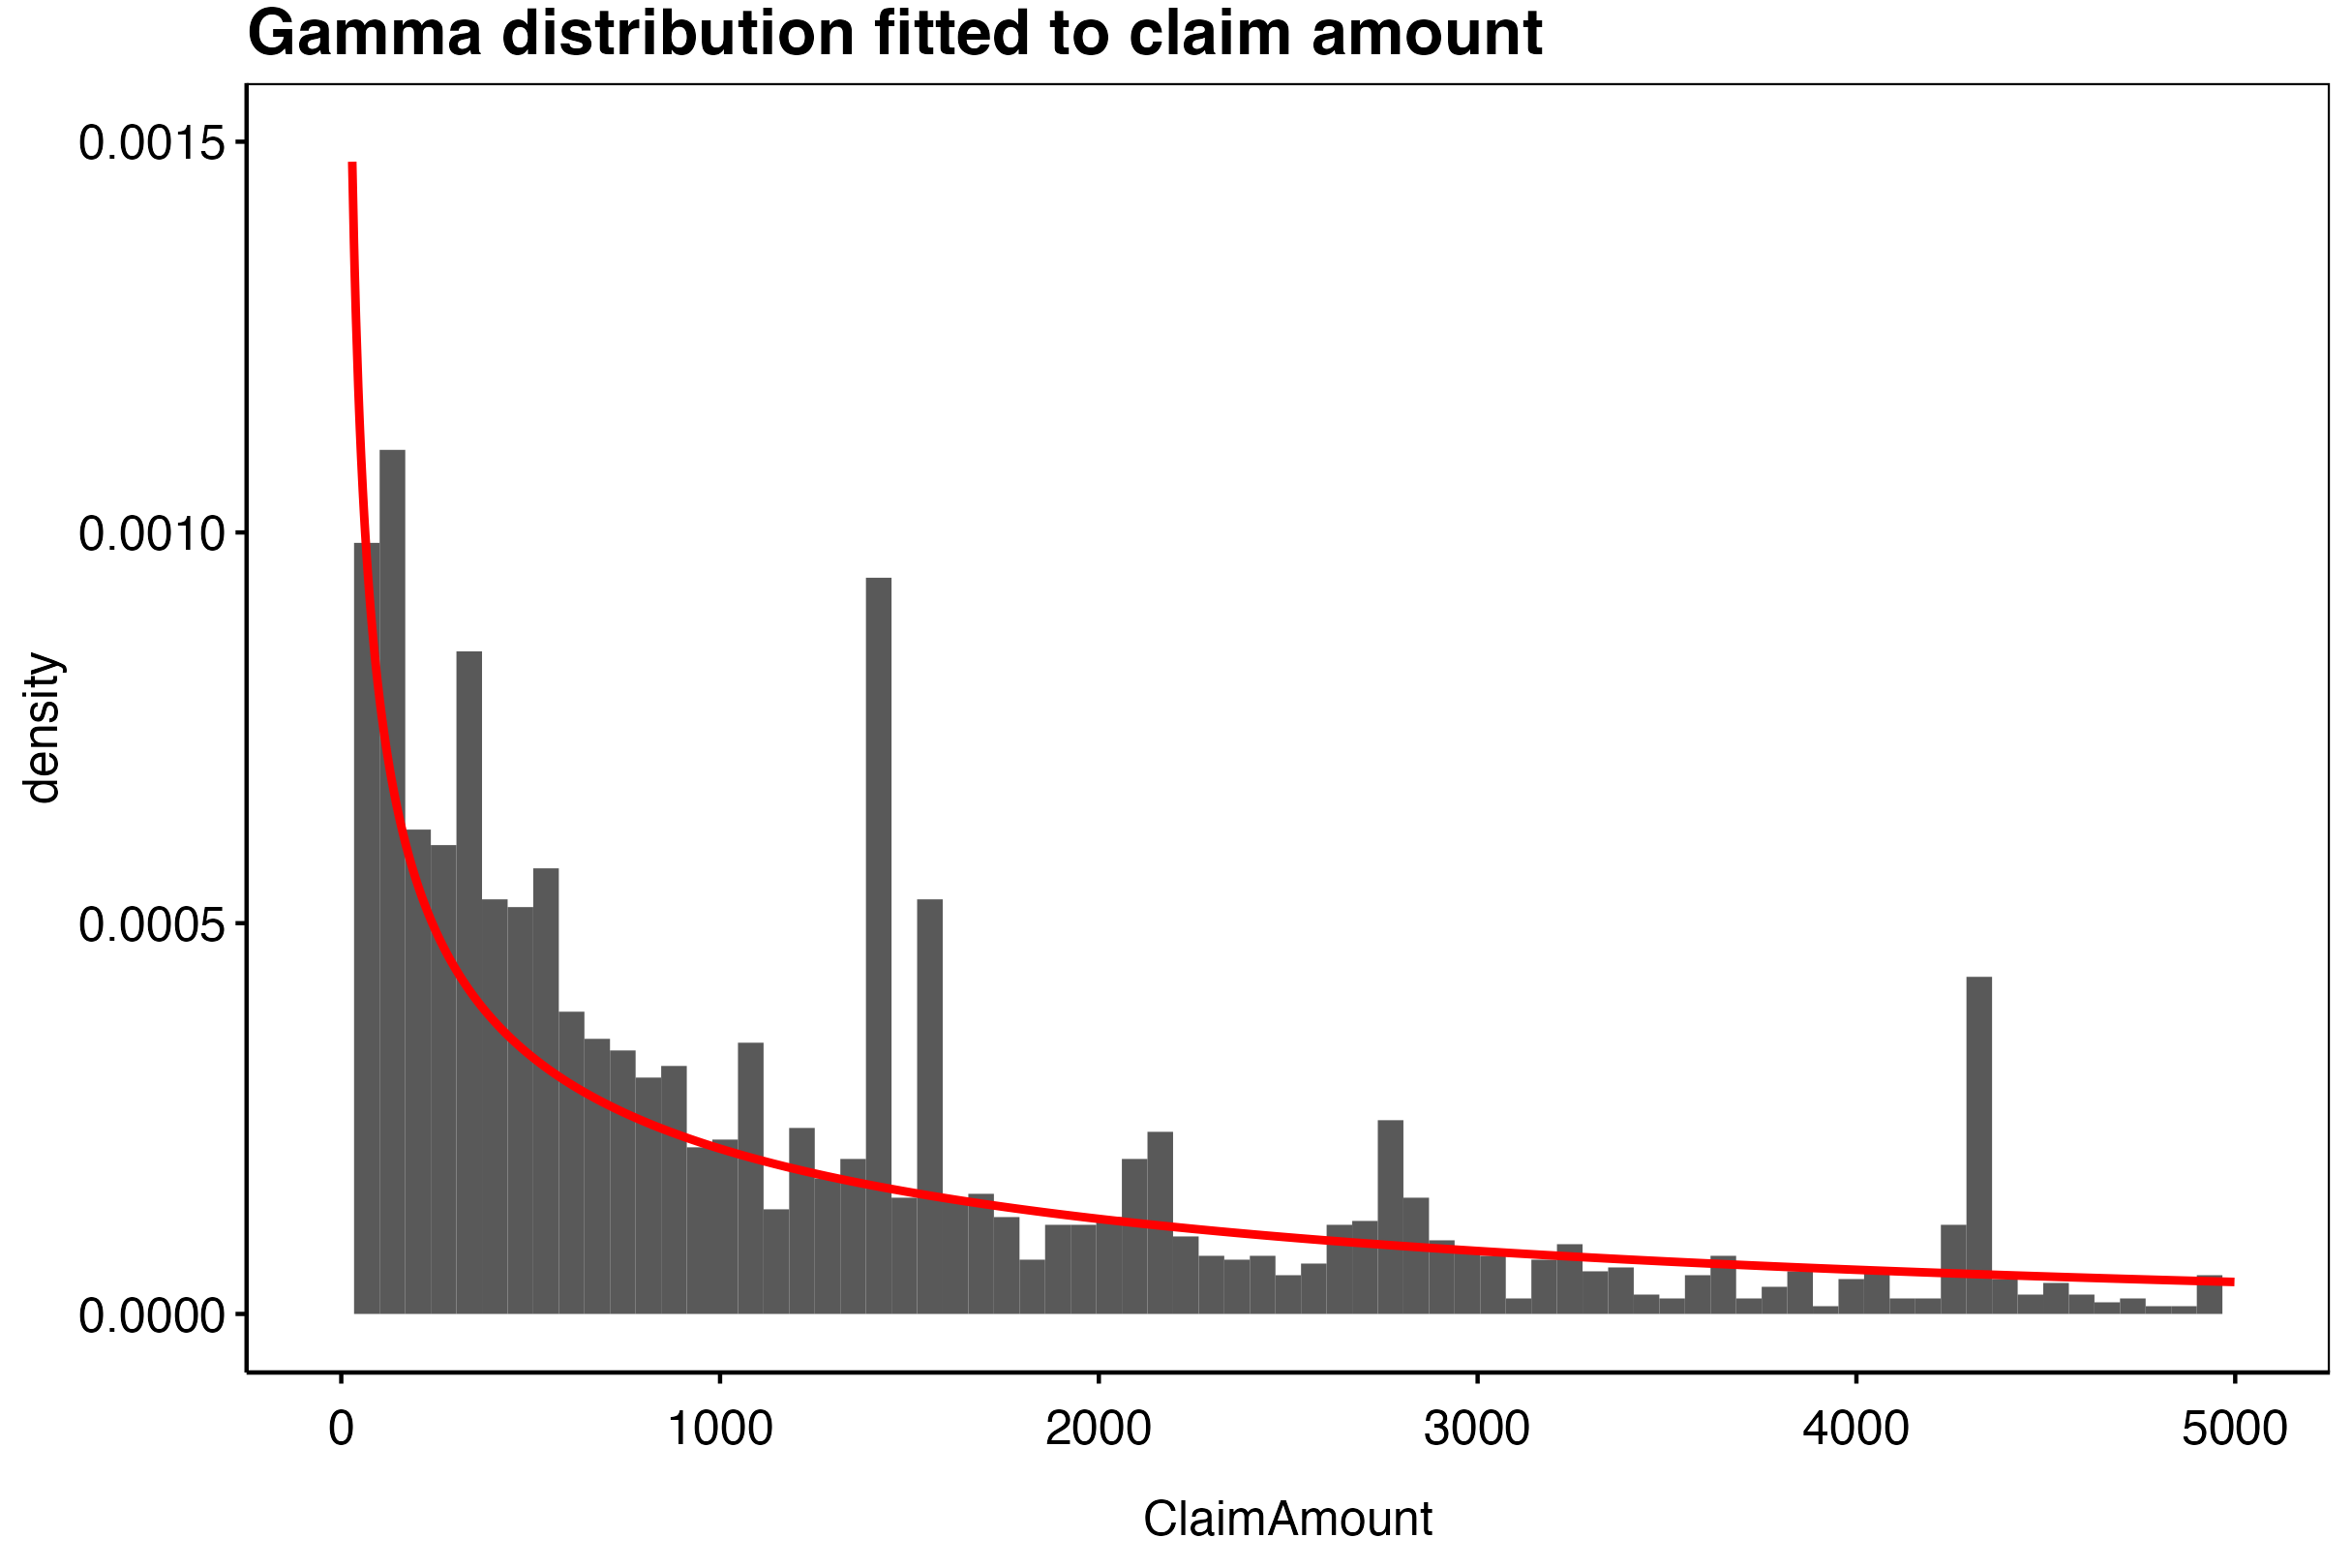
\includegraphics[width=0.75\textwidth]{figures/sev_gamma.png}
\end{figure}

One may fit samples \(X_1,...,X_N\) of iid \(\Gamma(\alpha,\beta)\)
distributed variables using MLE methods. In this notation we have
\(\alpha>0\) being the shape parameter and \(\beta > 0\) being the rate.
One may calculate an estimate of \(\alpha\) and \(\beta\) using:

\[
\hat\alpha_N=\frac{N\sum_{i=1}^NX_i}{N\sum_{i=1}^N\log(X_i)X_i-\left(\sum_{i=1}^NX_i\right)\left(\sum_{i=1}^N\log(X_i)\right)}
\]

and

\[
\frac{1}{\hat\beta_N}=\frac{1}{N^2}\left(N\sum_{i=1}^N\log(X_i)X_i-\left(\sum_{i=1}^NX_i\right)\left(\sum_{i=1}^N\log(X_i)\right)\right).
\]

\end{document}